\documentclass[twoside]{book}

% Packages required by doxygen
\usepackage{fixltx2e}
\usepackage{calc}
\usepackage{doxygen}
\usepackage[export]{adjustbox} % also loads graphicx
\usepackage{graphicx}
\usepackage[utf8]{inputenc}
\usepackage{makeidx}
\usepackage{multicol}
\usepackage{multirow}
\PassOptionsToPackage{warn}{textcomp}
\usepackage{textcomp}
\usepackage[nointegrals]{wasysym}
\usepackage[table]{xcolor}

% Font selection
\usepackage[T1]{fontenc}
\usepackage[scaled=.90]{helvet}
\usepackage{courier}
\usepackage{amssymb}
\usepackage{sectsty}
\renewcommand{\familydefault}{\sfdefault}
\allsectionsfont{%
  \fontseries{bc}\selectfont%
  \color{darkgray}%
}
\renewcommand{\DoxyLabelFont}{%
  \fontseries{bc}\selectfont%
  \color{darkgray}%
}
\newcommand{\+}{\discretionary{\mbox{\scriptsize$\hookleftarrow$}}{}{}}

% Page & text layout
\usepackage{geometry}
\geometry{%
  a4paper,%
  top=2.5cm,%
  bottom=2.5cm,%
  left=2.5cm,%
  right=2.5cm%
}
\tolerance=750
\hfuzz=15pt
\hbadness=750
\setlength{\emergencystretch}{15pt}
\setlength{\parindent}{0cm}
\setlength{\parskip}{3ex plus 2ex minus 2ex}
\makeatletter
\renewcommand{\paragraph}{%
  \@startsection{paragraph}{4}{0ex}{-1.0ex}{1.0ex}{%
    \normalfont\normalsize\bfseries\SS@parafont%
  }%
}
\renewcommand{\subparagraph}{%
  \@startsection{subparagraph}{5}{0ex}{-1.0ex}{1.0ex}{%
    \normalfont\normalsize\bfseries\SS@subparafont%
  }%
}
\makeatother

% Headers & footers
\usepackage{fancyhdr}
\pagestyle{fancyplain}
\fancyhead[LE]{\fancyplain{}{\bfseries\thepage}}
\fancyhead[CE]{\fancyplain{}{}}
\fancyhead[RE]{\fancyplain{}{\bfseries\leftmark}}
\fancyhead[LO]{\fancyplain{}{\bfseries\rightmark}}
\fancyhead[CO]{\fancyplain{}{}}
\fancyhead[RO]{\fancyplain{}{\bfseries\thepage}}
\fancyfoot[LE]{\fancyplain{}{}}
\fancyfoot[CE]{\fancyplain{}{}}
\fancyfoot[RE]{\fancyplain{}{\bfseries\scriptsize Generated by Doxygen }}
\fancyfoot[LO]{\fancyplain{}{\bfseries\scriptsize Generated by Doxygen }}
\fancyfoot[CO]{\fancyplain{}{}}
\fancyfoot[RO]{\fancyplain{}{}}
\renewcommand{\footrulewidth}{0.4pt}
\renewcommand{\chaptermark}[1]{%
  \markboth{#1}{}%
}
\renewcommand{\sectionmark}[1]{%
  \markright{\thesection\ #1}%
}

% Indices & bibliography
\usepackage{natbib}
\usepackage[titles]{tocloft}
\setcounter{tocdepth}{3}
\setcounter{secnumdepth}{5}
\makeindex

% Hyperlinks (required, but should be loaded last)
\usepackage{ifpdf}
\ifpdf
  \usepackage[pdftex,pagebackref=true]{hyperref}
\else
  \usepackage[ps2pdf,pagebackref=true]{hyperref}
\fi
\hypersetup{%
  colorlinks=true,%
  linkcolor=blue,%
  citecolor=blue,%
  unicode%
}

% Custom commands
\newcommand{\clearemptydoublepage}{%
  \newpage{\pagestyle{empty}\cleardoublepage}%
}

\usepackage{caption}
\captionsetup{labelsep=space,justification=centering,font={bf},singlelinecheck=off,skip=4pt,position=top}

%===== C O N T E N T S =====

\begin{document}

% Titlepage & ToC
\hypersetup{pageanchor=false,
             bookmarksnumbered=true,
             pdfencoding=unicode
            }
\pagenumbering{alph}
\begin{titlepage}
\vspace*{7cm}
\begin{center}%
{\Large My Project }\\
\vspace*{1cm}
{\large Generated by Doxygen 1.8.13}\\
\end{center}
\end{titlepage}
\clearemptydoublepage
\pagenumbering{roman}
\tableofcontents
\clearemptydoublepage
\pagenumbering{arabic}
\hypersetup{pageanchor=true}

%--- Begin generated contents ---
\chapter{Class Index}
\section{Class List}
Here are the classes, structs, unions and interfaces with brief descriptions\+:\begin{DoxyCompactList}
\item\contentsline{section}{\hyperlink{classBird}{Bird} }{\pageref{classBird}}{}
\item\contentsline{section}{\hyperlink{classOctree_1_1Callback}{Octree$<$ N $>$\+::\+Callback} }{\pageref{classOctree_1_1Callback}}{}
\item\contentsline{section}{\hyperlink{structBird_1_1compare}{Bird\+::compare} }{\pageref{structBird_1_1compare}}{}
\item\contentsline{section}{\hyperlink{classFlock}{Flock} }{\pageref{classFlock}}{}
\item\contentsline{section}{\hyperlink{classOctree_1_1Iterator}{Octree$<$ N $>$\+::\+Iterator} }{\pageref{classOctree_1_1Iterator}}{}
\item\contentsline{section}{\hyperlink{structNode}{Node} }{\pageref{structNode}}{}
\item\contentsline{section}{\hyperlink{classOctree}{Octree$<$ N $>$} }{\pageref{classOctree}}{}
\item\contentsline{section}{\hyperlink{structOctree_1_1OctreeNode}{Octree$<$ N $>$\+::\+Octree\+Node} }{\pageref{structOctree_1_1OctreeNode}}{}
\item\contentsline{section}{\hyperlink{structOctree_1_1Point}{Octree$<$ N $>$\+::\+Point} }{\pageref{structOctree_1_1Point}}{}
\item\contentsline{section}{\hyperlink{classsimulTimer}{simul\+Timer} }{\pageref{classsimulTimer}}{}
\end{DoxyCompactList}

\chapter{File Index}
\section{File List}
Here is a list of all files with brief descriptions\+:\begin{DoxyCompactList}
\item\contentsline{section}{\hyperlink{bird_8cpp}{bird.\+cpp} }{\pageref{bird_8cpp}}{}
\item\contentsline{section}{\hyperlink{bird_8h}{bird.\+h} }{\pageref{bird_8h}}{}
\item\contentsline{section}{\hyperlink{flock_8cpp}{flock.\+cpp} }{\pageref{flock_8cpp}}{}
\item\contentsline{section}{\hyperlink{flock_8h}{flock.\+h} }{\pageref{flock_8h}}{}
\item\contentsline{section}{\hyperlink{main_8cpp}{main.\+cpp} }{\pageref{main_8cpp}}{}
\item\contentsline{section}{\hyperlink{objloader_8cpp}{objloader.\+cpp} }{\pageref{objloader_8cpp}}{}
\item\contentsline{section}{\hyperlink{objloader_8hpp}{objloader.\+hpp} }{\pageref{objloader_8hpp}}{}
\item\contentsline{section}{\hyperlink{Octree_8h}{Octree.\+h} }{\pageref{Octree_8h}}{}
\item\contentsline{section}{\hyperlink{shader_8cpp}{shader.\+cpp} }{\pageref{shader_8cpp}}{}
\item\contentsline{section}{\hyperlink{shader_8hpp}{shader.\+hpp} }{\pageref{shader_8hpp}}{}
\item\contentsline{section}{\hyperlink{simulTimer_8cpp}{simul\+Timer.\+cpp} }{\pageref{simulTimer_8cpp}}{}
\item\contentsline{section}{\hyperlink{simulTimer_8h}{simul\+Timer.\+h} }{\pageref{simulTimer_8h}}{}
\item\contentsline{section}{\hyperlink{texture_8cpp}{texture.\+cpp} }{\pageref{texture_8cpp}}{}
\item\contentsline{section}{\hyperlink{texture_8hpp}{texture.\+hpp} }{\pageref{texture_8hpp}}{}
\end{DoxyCompactList}

\chapter{Class Documentation}
\hypertarget{classBird}{}\section{Bird Class Reference}
\label{classBird}\index{Bird@{Bird}}


{\ttfamily \#include $<$bird.\+h$>$}

\subsection*{Classes}
\begin{DoxyCompactItemize}
\item 
struct \hyperlink{structBird_1_1compare}{compare}
\end{DoxyCompactItemize}
\subsection*{Public Member Functions}
\begin{DoxyCompactItemize}
\item 
\hyperlink{classBird_a7c1b36856fe3a89d6098ec2b8a10ae8d}{Bird} ()
\item 
void \hyperlink{classBird_a3ff2e32d861a71e89c1294e0e19e91de}{update} (double dt, glm\+::vec3 velocity)
\item 
glm\+::vec3 \hyperlink{classBird_a4611f1cf5c173562bb4c14fe719f20fa}{get\+Position} ()
\item 
glm\+::vec3 \hyperlink{classBird_ad212b0b56ce7a244c02c78811fcc7a7c}{get\+Forward} ()
\item 
glm\+::vec3 \hyperlink{classBird_ac2e4e44987731d67de77e2a18245024d}{get\+Velocity} ()
\item 
void \hyperlink{classBird_a17574e6ab712a32bec19ba9b709bf903}{add\+Velocity} ()
\item 
double \hyperlink{classBird_a25cc8f4de5f1662fa56001531608fac9}{get\+Power} ()
\item 
glm\+::vec3 \hyperlink{classBird_a7f02b8f1ed943dd812b483a6361d81e2}{separate} ()
\item 
glm\+::vec3 \hyperlink{classBird_a41caabaf3f9fb37d0583f6384f12d9a1}{aligment} ()
\item 
glm\+::vec3 \hyperlink{classBird_ae30d88996b92134ab8acb4105766a5cb}{cohesion} ()
\item 
glm\+::vec3 \hyperlink{classBird_a6383559729a95495285d246f910fe37e}{follow\+Target} ()
\item 
double \hyperlink{classBird_a29d1ab4b40b2f9394f575019e3f8a247}{get\+Rand} ()
\end{DoxyCompactItemize}
\subsection*{Public Attributes}
\begin{DoxyCompactItemize}
\item 
std\+::set$<$ \hyperlink{classBird}{Bird} $\ast$, \hyperlink{structBird_1_1compare}{compare} $>$ \hyperlink{classBird_a30992001074a4c312bfdb40a745dc3f8}{neighbours}
\item 
glm\+::vec3 \hyperlink{classBird_a752294b0f405f7efec1eb0c135ab236b}{m\+Target}
\end{DoxyCompactItemize}


\subsection{Constructor \& Destructor Documentation}
\mbox{\Hypertarget{classBird_a7c1b36856fe3a89d6098ec2b8a10ae8d}\label{classBird_a7c1b36856fe3a89d6098ec2b8a10ae8d}} 
\index{Bird@{Bird}!Bird@{Bird}}
\index{Bird@{Bird}!Bird@{Bird}}
\subsubsection{\texorpdfstring{Bird()}{Bird()}}
{\footnotesize\ttfamily Bird\+::\+Bird (\begin{DoxyParamCaption}{ }\end{DoxyParamCaption})}



\subsection{Member Function Documentation}
\mbox{\Hypertarget{classBird_a17574e6ab712a32bec19ba9b709bf903}\label{classBird_a17574e6ab712a32bec19ba9b709bf903}} 
\index{Bird@{Bird}!add\+Velocity@{add\+Velocity}}
\index{add\+Velocity@{add\+Velocity}!Bird@{Bird}}
\subsubsection{\texorpdfstring{add\+Velocity()}{addVelocity()}}
{\footnotesize\ttfamily void Bird\+::add\+Velocity (\begin{DoxyParamCaption}{ }\end{DoxyParamCaption})}

\mbox{\Hypertarget{classBird_a41caabaf3f9fb37d0583f6384f12d9a1}\label{classBird_a41caabaf3f9fb37d0583f6384f12d9a1}} 
\index{Bird@{Bird}!aligment@{aligment}}
\index{aligment@{aligment}!Bird@{Bird}}
\subsubsection{\texorpdfstring{aligment()}{aligment()}}
{\footnotesize\ttfamily glm\+::vec3 Bird\+::aligment (\begin{DoxyParamCaption}{ }\end{DoxyParamCaption})}

\mbox{\Hypertarget{classBird_ae30d88996b92134ab8acb4105766a5cb}\label{classBird_ae30d88996b92134ab8acb4105766a5cb}} 
\index{Bird@{Bird}!cohesion@{cohesion}}
\index{cohesion@{cohesion}!Bird@{Bird}}
\subsubsection{\texorpdfstring{cohesion()}{cohesion()}}
{\footnotesize\ttfamily glm\+::vec3 Bird\+::cohesion (\begin{DoxyParamCaption}{ }\end{DoxyParamCaption})}

\mbox{\Hypertarget{classBird_a6383559729a95495285d246f910fe37e}\label{classBird_a6383559729a95495285d246f910fe37e}} 
\index{Bird@{Bird}!follow\+Target@{follow\+Target}}
\index{follow\+Target@{follow\+Target}!Bird@{Bird}}
\subsubsection{\texorpdfstring{follow\+Target()}{followTarget()}}
{\footnotesize\ttfamily glm\+::vec3 Bird\+::follow\+Target (\begin{DoxyParamCaption}{ }\end{DoxyParamCaption})}

\mbox{\Hypertarget{classBird_ad212b0b56ce7a244c02c78811fcc7a7c}\label{classBird_ad212b0b56ce7a244c02c78811fcc7a7c}} 
\index{Bird@{Bird}!get\+Forward@{get\+Forward}}
\index{get\+Forward@{get\+Forward}!Bird@{Bird}}
\subsubsection{\texorpdfstring{get\+Forward()}{getForward()}}
{\footnotesize\ttfamily glm\+::vec3 Bird\+::get\+Forward (\begin{DoxyParamCaption}{ }\end{DoxyParamCaption})}

\mbox{\Hypertarget{classBird_a4611f1cf5c173562bb4c14fe719f20fa}\label{classBird_a4611f1cf5c173562bb4c14fe719f20fa}} 
\index{Bird@{Bird}!get\+Position@{get\+Position}}
\index{get\+Position@{get\+Position}!Bird@{Bird}}
\subsubsection{\texorpdfstring{get\+Position()}{getPosition()}}
{\footnotesize\ttfamily glm\+::vec3 Bird\+::get\+Position (\begin{DoxyParamCaption}{ }\end{DoxyParamCaption})}

\mbox{\Hypertarget{classBird_a25cc8f4de5f1662fa56001531608fac9}\label{classBird_a25cc8f4de5f1662fa56001531608fac9}} 
\index{Bird@{Bird}!get\+Power@{get\+Power}}
\index{get\+Power@{get\+Power}!Bird@{Bird}}
\subsubsection{\texorpdfstring{get\+Power()}{getPower()}}
{\footnotesize\ttfamily double Bird\+::get\+Power (\begin{DoxyParamCaption}{ }\end{DoxyParamCaption})}

\mbox{\Hypertarget{classBird_a29d1ab4b40b2f9394f575019e3f8a247}\label{classBird_a29d1ab4b40b2f9394f575019e3f8a247}} 
\index{Bird@{Bird}!get\+Rand@{get\+Rand}}
\index{get\+Rand@{get\+Rand}!Bird@{Bird}}
\subsubsection{\texorpdfstring{get\+Rand()}{getRand()}}
{\footnotesize\ttfamily double Bird\+::get\+Rand (\begin{DoxyParamCaption}{ }\end{DoxyParamCaption})}

\mbox{\Hypertarget{classBird_ac2e4e44987731d67de77e2a18245024d}\label{classBird_ac2e4e44987731d67de77e2a18245024d}} 
\index{Bird@{Bird}!get\+Velocity@{get\+Velocity}}
\index{get\+Velocity@{get\+Velocity}!Bird@{Bird}}
\subsubsection{\texorpdfstring{get\+Velocity()}{getVelocity()}}
{\footnotesize\ttfamily glm\+::vec3 Bird\+::get\+Velocity (\begin{DoxyParamCaption}{ }\end{DoxyParamCaption})}

\mbox{\Hypertarget{classBird_a7f02b8f1ed943dd812b483a6361d81e2}\label{classBird_a7f02b8f1ed943dd812b483a6361d81e2}} 
\index{Bird@{Bird}!separate@{separate}}
\index{separate@{separate}!Bird@{Bird}}
\subsubsection{\texorpdfstring{separate()}{separate()}}
{\footnotesize\ttfamily glm\+::vec3 Bird\+::separate (\begin{DoxyParamCaption}{ }\end{DoxyParamCaption})}

\mbox{\Hypertarget{classBird_a3ff2e32d861a71e89c1294e0e19e91de}\label{classBird_a3ff2e32d861a71e89c1294e0e19e91de}} 
\index{Bird@{Bird}!update@{update}}
\index{update@{update}!Bird@{Bird}}
\subsubsection{\texorpdfstring{update()}{update()}}
{\footnotesize\ttfamily void Bird\+::update (\begin{DoxyParamCaption}\item[{double}]{dt,  }\item[{glm\+::vec3}]{velocity }\end{DoxyParamCaption})}



\subsection{Member Data Documentation}
\mbox{\Hypertarget{classBird_a752294b0f405f7efec1eb0c135ab236b}\label{classBird_a752294b0f405f7efec1eb0c135ab236b}} 
\index{Bird@{Bird}!m\+Target@{m\+Target}}
\index{m\+Target@{m\+Target}!Bird@{Bird}}
\subsubsection{\texorpdfstring{m\+Target}{mTarget}}
{\footnotesize\ttfamily glm\+::vec3 Bird\+::m\+Target}

\mbox{\Hypertarget{classBird_a30992001074a4c312bfdb40a745dc3f8}\label{classBird_a30992001074a4c312bfdb40a745dc3f8}} 
\index{Bird@{Bird}!neighbours@{neighbours}}
\index{neighbours@{neighbours}!Bird@{Bird}}
\subsubsection{\texorpdfstring{neighbours}{neighbours}}
{\footnotesize\ttfamily std\+::set$<$\hyperlink{classBird}{Bird}$\ast$,\hyperlink{structBird_1_1compare}{compare}$>$ Bird\+::neighbours}



The documentation for this class was generated from the following files\+:\begin{DoxyCompactItemize}
\item 
\hyperlink{bird_8h}{bird.\+h}\item 
\hyperlink{bird_8cpp}{bird.\+cpp}\end{DoxyCompactItemize}

\hypertarget{classOctree_1_1Callback}{}\section{Octree$<$ N $>$\+:\+:Callback Class Reference}
\label{classOctree_1_1Callback}\index{Octree$<$ N $>$\+::\+Callback@{Octree$<$ N $>$\+::\+Callback}}


{\ttfamily \#include $<$Octree.\+h$>$}

\subsection*{Public Member Functions}
\begin{DoxyCompactItemize}
\item 
virtual bool \hyperlink{classOctree_1_1Callback_a0d944e37207b2171d3f014912fe2f1f9}{operator()} (const float min\mbox{[}3\mbox{]}, const float max\mbox{[}3\mbox{]}, N \&node\+Data)=0
\end{DoxyCompactItemize}


\subsection{Member Function Documentation}
\mbox{\Hypertarget{classOctree_1_1Callback_a0d944e37207b2171d3f014912fe2f1f9}\label{classOctree_1_1Callback_a0d944e37207b2171d3f014912fe2f1f9}} 
\index{Octree\+::\+Callback@{Octree\+::\+Callback}!operator()@{operator()}}
\index{operator()@{operator()}!Octree\+::\+Callback@{Octree\+::\+Callback}}
\subsubsection{\texorpdfstring{operator()()}{operator()()}}
{\footnotesize\ttfamily template$<$class N$>$ \\
virtual bool \hyperlink{classOctree}{Octree}$<$ N $>$\+::Callback\+::operator() (\begin{DoxyParamCaption}\item[{const float}]{min\mbox{[}3\mbox{]},  }\item[{const float}]{max\mbox{[}3\mbox{]},  }\item[{N \&}]{node\+Data }\end{DoxyParamCaption})\hspace{0.3cm}{\ttfamily [pure virtual]}}



The documentation for this class was generated from the following file\+:\begin{DoxyCompactItemize}
\item 
\hyperlink{Octree_8h}{Octree.\+h}\end{DoxyCompactItemize}

\hypertarget{structBird_1_1compare}{}\section{Bird\+:\+:compare Struct Reference}
\label{structBird_1_1compare}\index{Bird\+::compare@{Bird\+::compare}}


{\ttfamily \#include $<$bird.\+h$>$}

\subsection*{Public Member Functions}
\begin{DoxyCompactItemize}
\item 
bool \hyperlink{structBird_1_1compare_a4c828e376650a2c8767edd0e09f93bbe}{operator()} (\hyperlink{classBird}{Bird} $\ast$a, \hyperlink{classBird}{Bird} $\ast$b)
\end{DoxyCompactItemize}


\subsection{Member Function Documentation}
\mbox{\Hypertarget{structBird_1_1compare_a4c828e376650a2c8767edd0e09f93bbe}\label{structBird_1_1compare_a4c828e376650a2c8767edd0e09f93bbe}} 
\index{Bird\+::compare@{Bird\+::compare}!operator()@{operator()}}
\index{operator()@{operator()}!Bird\+::compare@{Bird\+::compare}}
\subsubsection{\texorpdfstring{operator()()}{operator()()}}
{\footnotesize\ttfamily bool Bird\+::compare\+::operator() (\begin{DoxyParamCaption}\item[{\hyperlink{classBird}{Bird} $\ast$}]{a,  }\item[{\hyperlink{classBird}{Bird} $\ast$}]{b }\end{DoxyParamCaption})\hspace{0.3cm}{\ttfamily [inline]}}



The documentation for this struct was generated from the following file\+:\begin{DoxyCompactItemize}
\item 
\hyperlink{bird_8h}{bird.\+h}\end{DoxyCompactItemize}

\hypertarget{classFlock}{}\section{Flock Class Reference}
\label{classFlock}\index{Flock@{Flock}}


{\ttfamily \#include $<$flock.\+h$>$}



Collaboration diagram for Flock\+:
\nopagebreak
\begin{figure}[H]
\begin{center}
\leavevmode
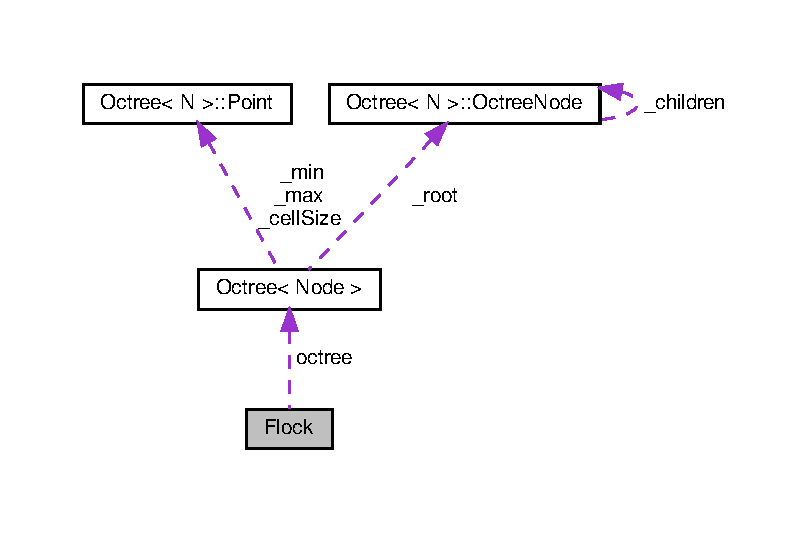
\includegraphics[width=350pt]{classFlock__coll__graph}
\end{center}
\end{figure}
\subsection*{Public Member Functions}
\begin{DoxyCompactItemize}
\item 
\hyperlink{classFlock_a2a0a514c368e21f718ad7358ed42f3b7}{Flock} ()
\item 
void \hyperlink{classFlock_a2bc42b2940b1ef99c120f58ee7918775}{add} (\hyperlink{classBird}{Bird} $\ast$b)
\item 
void \hyperlink{classFlock_aba009392cab937cd3911278a56c12bfc}{update} (double dt, float \hyperlink{main_8cpp_a3d47f7e2bf80c3044a1c4fb985d08565}{separation}, float \hyperlink{main_8cpp_a9b609437b0a9c5266747f6a31b8bf90e}{alignment}, float \hyperlink{main_8cpp_ab665ec90cc49c91ed2d1e7e0ca3c386e}{cohesion}, float \hyperlink{main_8cpp_af0df2177301e4061ab72ade2ea437bcd}{target}, bool \hyperlink{main_8cpp_aae9e26fee26af7722250e6b27dbdf37a}{target\+\_\+present})
\item 
void \hyperlink{classFlock_abb8739e196b8d11699f06d9670c1768b}{update\+Targets} ()
\item 
void \hyperlink{classFlock_a8657b4c8affd9ad6a87c119f592baccb}{create\+Octree} ()
\item 
void \hyperlink{classFlock_a597ecc4f44495e610c7ff516d94ca560}{update\+Neighbours} ()
\item 
double \hyperlink{classFlock_a9c91990979a1d4cab91c5abd1d3ac983}{get\+Rand} ()
\item 
double \hyperlink{classFlock_a65ae41c2c0eaaab0498c5a091d63a776}{get\+Average\+Power} ()
\end{DoxyCompactItemize}
\subsection*{Public Attributes}
\begin{DoxyCompactItemize}
\item 
std\+::vector$<$ \hyperlink{classBird}{Bird} $\ast$ $>$ \hyperlink{classFlock_ad742a7776e824da6281031d7d9d88d0c}{m\+Birds}
\item 
\hyperlink{classOctree}{Octree}$<$ \hyperlink{structNode}{Node} $>$ $\ast$ \hyperlink{classFlock_a1e280f2ca46cd9c68dc31c5e3d8fec2c}{octree}
\end{DoxyCompactItemize}


\subsection{Constructor \& Destructor Documentation}
\mbox{\Hypertarget{classFlock_a2a0a514c368e21f718ad7358ed42f3b7}\label{classFlock_a2a0a514c368e21f718ad7358ed42f3b7}} 
\index{Flock@{Flock}!Flock@{Flock}}
\index{Flock@{Flock}!Flock@{Flock}}
\subsubsection{\texorpdfstring{Flock()}{Flock()}}
{\footnotesize\ttfamily Flock\+::\+Flock (\begin{DoxyParamCaption}{ }\end{DoxyParamCaption})}



\subsection{Member Function Documentation}
\mbox{\Hypertarget{classFlock_a2bc42b2940b1ef99c120f58ee7918775}\label{classFlock_a2bc42b2940b1ef99c120f58ee7918775}} 
\index{Flock@{Flock}!add@{add}}
\index{add@{add}!Flock@{Flock}}
\subsubsection{\texorpdfstring{add()}{add()}}
{\footnotesize\ttfamily void Flock\+::add (\begin{DoxyParamCaption}\item[{\hyperlink{classBird}{Bird} $\ast$}]{b }\end{DoxyParamCaption})}

\mbox{\Hypertarget{classFlock_a8657b4c8affd9ad6a87c119f592baccb}\label{classFlock_a8657b4c8affd9ad6a87c119f592baccb}} 
\index{Flock@{Flock}!create\+Octree@{create\+Octree}}
\index{create\+Octree@{create\+Octree}!Flock@{Flock}}
\subsubsection{\texorpdfstring{create\+Octree()}{createOctree()}}
{\footnotesize\ttfamily void Flock\+::create\+Octree (\begin{DoxyParamCaption}{ }\end{DoxyParamCaption})}

\mbox{\Hypertarget{classFlock_a65ae41c2c0eaaab0498c5a091d63a776}\label{classFlock_a65ae41c2c0eaaab0498c5a091d63a776}} 
\index{Flock@{Flock}!get\+Average\+Power@{get\+Average\+Power}}
\index{get\+Average\+Power@{get\+Average\+Power}!Flock@{Flock}}
\subsubsection{\texorpdfstring{get\+Average\+Power()}{getAveragePower()}}
{\footnotesize\ttfamily double Flock\+::get\+Average\+Power (\begin{DoxyParamCaption}{ }\end{DoxyParamCaption})}

\mbox{\Hypertarget{classFlock_a9c91990979a1d4cab91c5abd1d3ac983}\label{classFlock_a9c91990979a1d4cab91c5abd1d3ac983}} 
\index{Flock@{Flock}!get\+Rand@{get\+Rand}}
\index{get\+Rand@{get\+Rand}!Flock@{Flock}}
\subsubsection{\texorpdfstring{get\+Rand()}{getRand()}}
{\footnotesize\ttfamily double Flock\+::get\+Rand (\begin{DoxyParamCaption}{ }\end{DoxyParamCaption})}

\mbox{\Hypertarget{classFlock_aba009392cab937cd3911278a56c12bfc}\label{classFlock_aba009392cab937cd3911278a56c12bfc}} 
\index{Flock@{Flock}!update@{update}}
\index{update@{update}!Flock@{Flock}}
\subsubsection{\texorpdfstring{update()}{update()}}
{\footnotesize\ttfamily void Flock\+::update (\begin{DoxyParamCaption}\item[{double}]{dt,  }\item[{float}]{separation,  }\item[{float}]{alignment,  }\item[{float}]{cohesion,  }\item[{float}]{target,  }\item[{bool}]{target\+\_\+present }\end{DoxyParamCaption})}

\mbox{\Hypertarget{classFlock_a597ecc4f44495e610c7ff516d94ca560}\label{classFlock_a597ecc4f44495e610c7ff516d94ca560}} 
\index{Flock@{Flock}!update\+Neighbours@{update\+Neighbours}}
\index{update\+Neighbours@{update\+Neighbours}!Flock@{Flock}}
\subsubsection{\texorpdfstring{update\+Neighbours()}{updateNeighbours()}}
{\footnotesize\ttfamily void Flock\+::update\+Neighbours (\begin{DoxyParamCaption}{ }\end{DoxyParamCaption})}

\mbox{\Hypertarget{classFlock_abb8739e196b8d11699f06d9670c1768b}\label{classFlock_abb8739e196b8d11699f06d9670c1768b}} 
\index{Flock@{Flock}!update\+Targets@{update\+Targets}}
\index{update\+Targets@{update\+Targets}!Flock@{Flock}}
\subsubsection{\texorpdfstring{update\+Targets()}{updateTargets()}}
{\footnotesize\ttfamily void Flock\+::update\+Targets (\begin{DoxyParamCaption}{ }\end{DoxyParamCaption})}



\subsection{Member Data Documentation}
\mbox{\Hypertarget{classFlock_ad742a7776e824da6281031d7d9d88d0c}\label{classFlock_ad742a7776e824da6281031d7d9d88d0c}} 
\index{Flock@{Flock}!m\+Birds@{m\+Birds}}
\index{m\+Birds@{m\+Birds}!Flock@{Flock}}
\subsubsection{\texorpdfstring{m\+Birds}{mBirds}}
{\footnotesize\ttfamily std\+::vector$<$\hyperlink{classBird}{Bird}$\ast$$>$ Flock\+::m\+Birds}

\mbox{\Hypertarget{classFlock_a1e280f2ca46cd9c68dc31c5e3d8fec2c}\label{classFlock_a1e280f2ca46cd9c68dc31c5e3d8fec2c}} 
\index{Flock@{Flock}!octree@{octree}}
\index{octree@{octree}!Flock@{Flock}}
\subsubsection{\texorpdfstring{octree}{octree}}
{\footnotesize\ttfamily \hyperlink{classOctree}{Octree}$<$\hyperlink{structNode}{Node}$>$$\ast$ Flock\+::octree}



The documentation for this class was generated from the following files\+:\begin{DoxyCompactItemize}
\item 
\hyperlink{flock_8h}{flock.\+h}\item 
\hyperlink{flock_8cpp}{flock.\+cpp}\end{DoxyCompactItemize}

\hypertarget{classOctree_1_1Iterator}{}\section{Octree$<$ N $>$\+:\+:Iterator Class Reference}
\label{classOctree_1_1Iterator}\index{Octree$<$ N $>$\+::\+Iterator@{Octree$<$ N $>$\+::\+Iterator}}


{\ttfamily \#include $<$Octree.\+h$>$}



Collaboration diagram for Octree$<$ N $>$\+:\+:Iterator\+:
\nopagebreak
\begin{figure}[H]
\begin{center}
\leavevmode
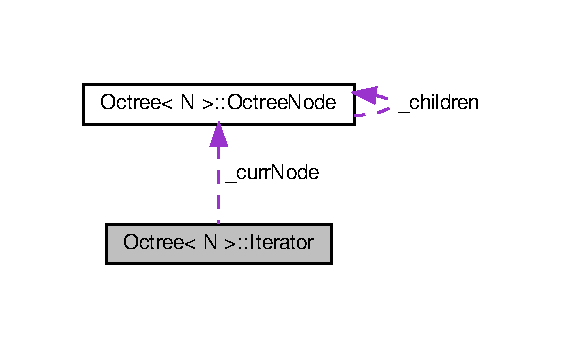
\includegraphics[width=271pt]{classOctree_1_1Iterator__coll__graph}
\end{center}
\end{figure}
\subsection*{Public Member Functions}
\begin{DoxyCompactItemize}
\item 
\hyperlink{classOctree_1_1Iterator}{Iterator} \hyperlink{classOctree_1_1Iterator_a967ccaaecd324ba6fbbd735d07d5bab8}{get\+Child} (int i)
\item 
N $\ast$ \hyperlink{classOctree_1_1Iterator_a507990201d4c1923cd137b2e1e75f1a9}{get\+Data} ()
\end{DoxyCompactItemize}
\subsection*{Protected Member Functions}
\begin{DoxyCompactItemize}
\item 
\hyperlink{classOctree_1_1Iterator_af4b294898f6586f90fbfd1aee3c42252}{Iterator} (\hyperlink{structOctree_1_1OctreeNode}{Octree\+Node} $\ast$node)
\end{DoxyCompactItemize}
\subsection*{Protected Attributes}
\begin{DoxyCompactItemize}
\item 
\hyperlink{structOctree_1_1OctreeNode}{Octree\+Node} $\ast$ \hyperlink{classOctree_1_1Iterator_ad8317eed660de125e9ecb2ea75a7e1ef}{\+\_\+curr\+Node}
\end{DoxyCompactItemize}
\subsection*{Friends}
\begin{DoxyCompactItemize}
\item 
class \hyperlink{classOctree_1_1Iterator_acc8a7ec8cf44f290482ad3d68f6a7719}{Octree}
\end{DoxyCompactItemize}


\subsection{Constructor \& Destructor Documentation}
\mbox{\Hypertarget{classOctree_1_1Iterator_af4b294898f6586f90fbfd1aee3c42252}\label{classOctree_1_1Iterator_af4b294898f6586f90fbfd1aee3c42252}} 
\index{Octree\+::\+Iterator@{Octree\+::\+Iterator}!Iterator@{Iterator}}
\index{Iterator@{Iterator}!Octree\+::\+Iterator@{Octree\+::\+Iterator}}
\subsubsection{\texorpdfstring{Iterator()}{Iterator()}}
{\footnotesize\ttfamily template$<$class N$>$ \\
\hyperlink{classOctree}{Octree}$<$ N $>$\+::Iterator\+::\+Iterator (\begin{DoxyParamCaption}\item[{\hyperlink{structOctree_1_1OctreeNode}{Octree\+Node} $\ast$}]{node }\end{DoxyParamCaption})\hspace{0.3cm}{\ttfamily [inline]}, {\ttfamily [protected]}}



\subsection{Member Function Documentation}
\mbox{\Hypertarget{classOctree_1_1Iterator_a967ccaaecd324ba6fbbd735d07d5bab8}\label{classOctree_1_1Iterator_a967ccaaecd324ba6fbbd735d07d5bab8}} 
\index{Octree\+::\+Iterator@{Octree\+::\+Iterator}!get\+Child@{get\+Child}}
\index{get\+Child@{get\+Child}!Octree\+::\+Iterator@{Octree\+::\+Iterator}}
\subsubsection{\texorpdfstring{get\+Child()}{getChild()}}
{\footnotesize\ttfamily template$<$class N$>$ \\
\hyperlink{classOctree_1_1Iterator}{Iterator} \hyperlink{classOctree}{Octree}$<$ N $>$\+::Iterator\+::get\+Child (\begin{DoxyParamCaption}\item[{int}]{i }\end{DoxyParamCaption})\hspace{0.3cm}{\ttfamily [inline]}}

\mbox{\Hypertarget{classOctree_1_1Iterator_a507990201d4c1923cd137b2e1e75f1a9}\label{classOctree_1_1Iterator_a507990201d4c1923cd137b2e1e75f1a9}} 
\index{Octree\+::\+Iterator@{Octree\+::\+Iterator}!get\+Data@{get\+Data}}
\index{get\+Data@{get\+Data}!Octree\+::\+Iterator@{Octree\+::\+Iterator}}
\subsubsection{\texorpdfstring{get\+Data()}{getData()}}
{\footnotesize\ttfamily template$<$class N$>$ \\
N$\ast$ \hyperlink{classOctree}{Octree}$<$ N $>$\+::Iterator\+::get\+Data (\begin{DoxyParamCaption}{ }\end{DoxyParamCaption})\hspace{0.3cm}{\ttfamily [inline]}}



\subsection{Friends And Related Function Documentation}
\mbox{\Hypertarget{classOctree_1_1Iterator_acc8a7ec8cf44f290482ad3d68f6a7719}\label{classOctree_1_1Iterator_acc8a7ec8cf44f290482ad3d68f6a7719}} 
\index{Octree\+::\+Iterator@{Octree\+::\+Iterator}!Octree@{Octree}}
\index{Octree@{Octree}!Octree\+::\+Iterator@{Octree\+::\+Iterator}}
\subsubsection{\texorpdfstring{Octree}{Octree}}
{\footnotesize\ttfamily template$<$class N$>$ \\
friend class \hyperlink{classOctree}{Octree}\hspace{0.3cm}{\ttfamily [friend]}}



\subsection{Member Data Documentation}
\mbox{\Hypertarget{classOctree_1_1Iterator_ad8317eed660de125e9ecb2ea75a7e1ef}\label{classOctree_1_1Iterator_ad8317eed660de125e9ecb2ea75a7e1ef}} 
\index{Octree\+::\+Iterator@{Octree\+::\+Iterator}!\+\_\+curr\+Node@{\+\_\+curr\+Node}}
\index{\+\_\+curr\+Node@{\+\_\+curr\+Node}!Octree\+::\+Iterator@{Octree\+::\+Iterator}}
\subsubsection{\texorpdfstring{\+\_\+curr\+Node}{\_currNode}}
{\footnotesize\ttfamily template$<$class N$>$ \\
\hyperlink{structOctree_1_1OctreeNode}{Octree\+Node}$\ast$ \hyperlink{classOctree}{Octree}$<$ N $>$\+::Iterator\+::\+\_\+curr\+Node\hspace{0.3cm}{\ttfamily [protected]}}



The documentation for this class was generated from the following file\+:\begin{DoxyCompactItemize}
\item 
\hyperlink{Octree_8h}{Octree.\+h}\end{DoxyCompactItemize}

\hypertarget{structNode}{}\section{Node Struct Reference}
\label{structNode}\index{Node@{Node}}


{\ttfamily \#include $<$flock.\+h$>$}

\subsection*{Public Attributes}
\begin{DoxyCompactItemize}
\item 
std\+::vector$<$ \hyperlink{classBird}{Bird} $\ast$ $>$ \hyperlink{structNode_a6649eb5fac4e4c97f592b823a5b113ed}{birds}
\end{DoxyCompactItemize}


\subsection{Member Data Documentation}
\mbox{\Hypertarget{structNode_a6649eb5fac4e4c97f592b823a5b113ed}\label{structNode_a6649eb5fac4e4c97f592b823a5b113ed}} 
\index{Node@{Node}!birds@{birds}}
\index{birds@{birds}!Node@{Node}}
\subsubsection{\texorpdfstring{birds}{birds}}
{\footnotesize\ttfamily std\+::vector$<$\hyperlink{classBird}{Bird}$\ast$$>$ Node\+::birds}



The documentation for this struct was generated from the following file\+:\begin{DoxyCompactItemize}
\item 
\hyperlink{flock_8h}{flock.\+h}\end{DoxyCompactItemize}

\hypertarget{classOctree}{}\section{Octree$<$ N $>$ Class Template Reference}
\label{classOctree}\index{Octree$<$ N $>$@{Octree$<$ N $>$}}


{\ttfamily \#include $<$Octree.\+h$>$}



Collaboration diagram for Octree$<$ N $>$\+:
\nopagebreak
\begin{figure}[H]
\begin{center}
\leavevmode
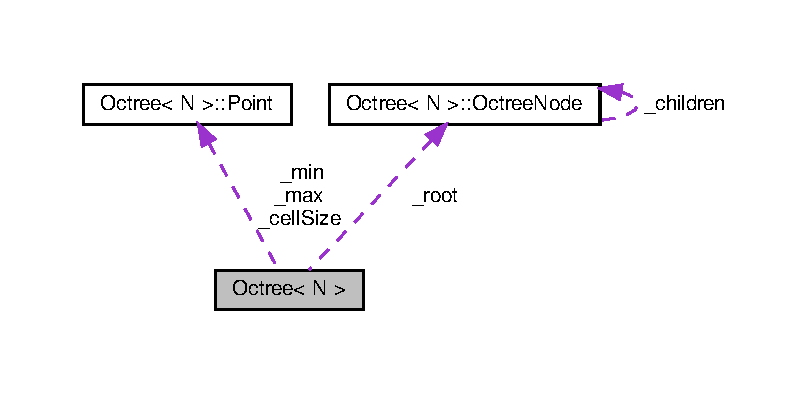
\includegraphics[width=350pt]{classOctree__coll__graph}
\end{center}
\end{figure}
\subsection*{Classes}
\begin{DoxyCompactItemize}
\item 
class \hyperlink{classOctree_1_1Callback}{Callback}
\item 
class \hyperlink{classOctree_1_1Iterator}{Iterator}
\item 
struct \hyperlink{structOctree_1_1OctreeNode}{Octree\+Node}
\item 
struct \hyperlink{structOctree_1_1Point}{Point}
\end{DoxyCompactItemize}
\subsection*{Public Member Functions}
\begin{DoxyCompactItemize}
\item 
\hyperlink{classOctree_aad1a0fd489e7412610b0161cff5da573}{Octree} (float min\mbox{[}3\mbox{]}, float max\mbox{[}3\mbox{]}, float cell\+Size\mbox{[}3\mbox{]})
\item 
virtual \hyperlink{classOctree_a7fb8884a9c9147da4020217f58237932}{$\sim$\+Octree} ()
\item 
N \& \hyperlink{classOctree_aeb0eeedf29f8c026ba53689def0c2f6b}{get\+Cell} (const float pos\mbox{[}3\mbox{]}, \hyperlink{classOctree_1_1Callback}{Callback} $\ast$callback=N\+U\+LL)
\item 
void \hyperlink{classOctree_a13d22bffc1be63deb3557c230ac5e17e}{traverse} (\hyperlink{classOctree_1_1Callback}{Callback} $\ast$callback)
\item 
void \hyperlink{classOctree_a4038c20a015dbf6b74fd9ccd76fb80cd}{clear} ()
\item 
\hyperlink{classOctree_1_1Iterator}{Iterator} \hyperlink{classOctree_ad2974d58fadff0b043d6e8b1828b509c}{get\+Iterator} ()
\end{DoxyCompactItemize}
\subsection*{Protected Member Functions}
\begin{DoxyCompactItemize}
\item 
void \hyperlink{classOctree_a2f7949797701cd01d398a76c323ec845}{traverse\+Recursive} (\hyperlink{classOctree_1_1Callback}{Callback} $\ast$callback, const \hyperlink{structOctree_1_1Point}{Point} \&curr\+Min, const \hyperlink{structOctree_1_1Point}{Point} \&curr\+Max, \hyperlink{structOctree_1_1OctreeNode}{Octree\+Node} $\ast$curr\+Node)
\end{DoxyCompactItemize}
\subsection*{Protected Attributes}
\begin{DoxyCompactItemize}
\item 
\hyperlink{structOctree_1_1Point}{Point} \hyperlink{classOctree_ab47cc9e63705799270956fc6f769c277}{\+\_\+min}
\item 
\hyperlink{structOctree_1_1Point}{Point} \hyperlink{classOctree_a58bcb3926893c3c8d463e05859fd600c}{\+\_\+max}
\item 
\hyperlink{structOctree_1_1Point}{Point} \hyperlink{classOctree_a6b398a3bf87d71dabc6b72180a551f0b}{\+\_\+cell\+Size}
\item 
\hyperlink{structOctree_1_1OctreeNode}{Octree\+Node} $\ast$ \hyperlink{classOctree_a1825458b3af1769fc9ce7021b8438574}{\+\_\+root}
\end{DoxyCompactItemize}


\subsection{Constructor \& Destructor Documentation}
\mbox{\Hypertarget{classOctree_aad1a0fd489e7412610b0161cff5da573}\label{classOctree_aad1a0fd489e7412610b0161cff5da573}} 
\index{Octree@{Octree}!Octree@{Octree}}
\index{Octree@{Octree}!Octree@{Octree}}
\subsubsection{\texorpdfstring{Octree()}{Octree()}}
{\footnotesize\ttfamily template$<$class N$>$ \\
\hyperlink{classOctree}{Octree}$<$ N $>$\+::\hyperlink{classOctree}{Octree} (\begin{DoxyParamCaption}\item[{float}]{min\mbox{[}3\mbox{]},  }\item[{float}]{max\mbox{[}3\mbox{]},  }\item[{float}]{cell\+Size\mbox{[}3\mbox{]} }\end{DoxyParamCaption})\hspace{0.3cm}{\ttfamily [inline]}}

\mbox{\Hypertarget{classOctree_a7fb8884a9c9147da4020217f58237932}\label{classOctree_a7fb8884a9c9147da4020217f58237932}} 
\index{Octree@{Octree}!````~Octree@{$\sim$\+Octree}}
\index{````~Octree@{$\sim$\+Octree}!Octree@{Octree}}
\subsubsection{\texorpdfstring{$\sim$\+Octree()}{~Octree()}}
{\footnotesize\ttfamily template$<$class N$>$ \\
virtual \hyperlink{classOctree}{Octree}$<$ N $>$\+::$\sim$\hyperlink{classOctree}{Octree} (\begin{DoxyParamCaption}{ }\end{DoxyParamCaption})\hspace{0.3cm}{\ttfamily [inline]}, {\ttfamily [virtual]}}



\subsection{Member Function Documentation}
\mbox{\Hypertarget{classOctree_a4038c20a015dbf6b74fd9ccd76fb80cd}\label{classOctree_a4038c20a015dbf6b74fd9ccd76fb80cd}} 
\index{Octree@{Octree}!clear@{clear}}
\index{clear@{clear}!Octree@{Octree}}
\subsubsection{\texorpdfstring{clear()}{clear()}}
{\footnotesize\ttfamily template$<$class N$>$ \\
void \hyperlink{classOctree}{Octree}$<$ N $>$\+::clear (\begin{DoxyParamCaption}{ }\end{DoxyParamCaption})\hspace{0.3cm}{\ttfamily [inline]}}

\mbox{\Hypertarget{classOctree_aeb0eeedf29f8c026ba53689def0c2f6b}\label{classOctree_aeb0eeedf29f8c026ba53689def0c2f6b}} 
\index{Octree@{Octree}!get\+Cell@{get\+Cell}}
\index{get\+Cell@{get\+Cell}!Octree@{Octree}}
\subsubsection{\texorpdfstring{get\+Cell()}{getCell()}}
{\footnotesize\ttfamily template$<$class N$>$ \\
N\& \hyperlink{classOctree}{Octree}$<$ N $>$\+::get\+Cell (\begin{DoxyParamCaption}\item[{const float}]{pos\mbox{[}3\mbox{]},  }\item[{\hyperlink{classOctree_1_1Callback}{Callback} $\ast$}]{callback = {\ttfamily NULL} }\end{DoxyParamCaption})\hspace{0.3cm}{\ttfamily [inline]}}

\mbox{\Hypertarget{classOctree_ad2974d58fadff0b043d6e8b1828b509c}\label{classOctree_ad2974d58fadff0b043d6e8b1828b509c}} 
\index{Octree@{Octree}!get\+Iterator@{get\+Iterator}}
\index{get\+Iterator@{get\+Iterator}!Octree@{Octree}}
\subsubsection{\texorpdfstring{get\+Iterator()}{getIterator()}}
{\footnotesize\ttfamily template$<$class N$>$ \\
\hyperlink{classOctree_1_1Iterator}{Iterator} \hyperlink{classOctree}{Octree}$<$ N $>$\+::get\+Iterator (\begin{DoxyParamCaption}{ }\end{DoxyParamCaption})\hspace{0.3cm}{\ttfamily [inline]}}

\mbox{\Hypertarget{classOctree_a13d22bffc1be63deb3557c230ac5e17e}\label{classOctree_a13d22bffc1be63deb3557c230ac5e17e}} 
\index{Octree@{Octree}!traverse@{traverse}}
\index{traverse@{traverse}!Octree@{Octree}}
\subsubsection{\texorpdfstring{traverse()}{traverse()}}
{\footnotesize\ttfamily template$<$class N$>$ \\
void \hyperlink{classOctree}{Octree}$<$ N $>$\+::traverse (\begin{DoxyParamCaption}\item[{\hyperlink{classOctree_1_1Callback}{Callback} $\ast$}]{callback }\end{DoxyParamCaption})\hspace{0.3cm}{\ttfamily [inline]}}

\mbox{\Hypertarget{classOctree_a2f7949797701cd01d398a76c323ec845}\label{classOctree_a2f7949797701cd01d398a76c323ec845}} 
\index{Octree@{Octree}!traverse\+Recursive@{traverse\+Recursive}}
\index{traverse\+Recursive@{traverse\+Recursive}!Octree@{Octree}}
\subsubsection{\texorpdfstring{traverse\+Recursive()}{traverseRecursive()}}
{\footnotesize\ttfamily template$<$class N$>$ \\
void \hyperlink{classOctree}{Octree}$<$ N $>$\+::traverse\+Recursive (\begin{DoxyParamCaption}\item[{\hyperlink{classOctree_1_1Callback}{Callback} $\ast$}]{callback,  }\item[{const \hyperlink{structOctree_1_1Point}{Point} \&}]{curr\+Min,  }\item[{const \hyperlink{structOctree_1_1Point}{Point} \&}]{curr\+Max,  }\item[{\hyperlink{structOctree_1_1OctreeNode}{Octree\+Node} $\ast$}]{curr\+Node }\end{DoxyParamCaption})\hspace{0.3cm}{\ttfamily [inline]}, {\ttfamily [protected]}}



\subsection{Member Data Documentation}
\mbox{\Hypertarget{classOctree_a6b398a3bf87d71dabc6b72180a551f0b}\label{classOctree_a6b398a3bf87d71dabc6b72180a551f0b}} 
\index{Octree@{Octree}!\+\_\+cell\+Size@{\+\_\+cell\+Size}}
\index{\+\_\+cell\+Size@{\+\_\+cell\+Size}!Octree@{Octree}}
\subsubsection{\texorpdfstring{\+\_\+cell\+Size}{\_cellSize}}
{\footnotesize\ttfamily template$<$class N$>$ \\
\hyperlink{structOctree_1_1Point}{Point} \hyperlink{classOctree}{Octree}$<$ N $>$\+::\+\_\+cell\+Size\hspace{0.3cm}{\ttfamily [protected]}}

\mbox{\Hypertarget{classOctree_a58bcb3926893c3c8d463e05859fd600c}\label{classOctree_a58bcb3926893c3c8d463e05859fd600c}} 
\index{Octree@{Octree}!\+\_\+max@{\+\_\+max}}
\index{\+\_\+max@{\+\_\+max}!Octree@{Octree}}
\subsubsection{\texorpdfstring{\+\_\+max}{\_max}}
{\footnotesize\ttfamily template$<$class N$>$ \\
\hyperlink{structOctree_1_1Point}{Point} \hyperlink{classOctree}{Octree}$<$ N $>$\+::\+\_\+max\hspace{0.3cm}{\ttfamily [protected]}}

\mbox{\Hypertarget{classOctree_ab47cc9e63705799270956fc6f769c277}\label{classOctree_ab47cc9e63705799270956fc6f769c277}} 
\index{Octree@{Octree}!\+\_\+min@{\+\_\+min}}
\index{\+\_\+min@{\+\_\+min}!Octree@{Octree}}
\subsubsection{\texorpdfstring{\+\_\+min}{\_min}}
{\footnotesize\ttfamily template$<$class N$>$ \\
\hyperlink{structOctree_1_1Point}{Point} \hyperlink{classOctree}{Octree}$<$ N $>$\+::\+\_\+min\hspace{0.3cm}{\ttfamily [protected]}}

\mbox{\Hypertarget{classOctree_a1825458b3af1769fc9ce7021b8438574}\label{classOctree_a1825458b3af1769fc9ce7021b8438574}} 
\index{Octree@{Octree}!\+\_\+root@{\+\_\+root}}
\index{\+\_\+root@{\+\_\+root}!Octree@{Octree}}
\subsubsection{\texorpdfstring{\+\_\+root}{\_root}}
{\footnotesize\ttfamily template$<$class N$>$ \\
\hyperlink{structOctree_1_1OctreeNode}{Octree\+Node}$\ast$ \hyperlink{classOctree}{Octree}$<$ N $>$\+::\+\_\+root\hspace{0.3cm}{\ttfamily [protected]}}



The documentation for this class was generated from the following file\+:\begin{DoxyCompactItemize}
\item 
\hyperlink{Octree_8h}{Octree.\+h}\end{DoxyCompactItemize}

\hypertarget{structOctree_1_1OctreeNode}{}\section{Octree$<$ N $>$\+:\+:Octree\+Node Struct Reference}
\label{structOctree_1_1OctreeNode}\index{Octree$<$ N $>$\+::\+Octree\+Node@{Octree$<$ N $>$\+::\+Octree\+Node}}


{\ttfamily \#include $<$Octree.\+h$>$}



Collaboration diagram for Octree$<$ N $>$\+:\+:Octree\+Node\+:
\nopagebreak
\begin{figure}[H]
\begin{center}
\leavevmode
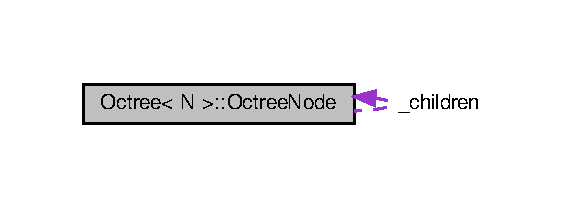
\includegraphics[width=271pt]{structOctree_1_1OctreeNode__coll__graph}
\end{center}
\end{figure}
\subsection*{Public Member Functions}
\begin{DoxyCompactItemize}
\item 
\hyperlink{structOctree_1_1OctreeNode_af85586ea3a494b59ebc0af118753dd69}{Octree\+Node} ()
\item 
virtual \hyperlink{structOctree_1_1OctreeNode_aabb39b4e83e43bacd5c4594aceb676bb}{$\sim$\+Octree\+Node} ()
\end{DoxyCompactItemize}
\subsection*{Public Attributes}
\begin{DoxyCompactItemize}
\item 
N \hyperlink{structOctree_1_1OctreeNode_acf3ff3707042ca6eaf42c6e1b5520376}{\+\_\+node\+Data}
\item 
\hyperlink{structOctree_1_1OctreeNode}{Octree\+Node} $\ast$ \hyperlink{structOctree_1_1OctreeNode_aba66f4dfb079ce3ec748889a7aa7e76d}{\+\_\+children} \mbox{[}8\mbox{]}
\end{DoxyCompactItemize}


\subsection{Constructor \& Destructor Documentation}
\mbox{\Hypertarget{structOctree_1_1OctreeNode_af85586ea3a494b59ebc0af118753dd69}\label{structOctree_1_1OctreeNode_af85586ea3a494b59ebc0af118753dd69}} 
\index{Octree\+::\+Octree\+Node@{Octree\+::\+Octree\+Node}!Octree\+Node@{Octree\+Node}}
\index{Octree\+Node@{Octree\+Node}!Octree\+::\+Octree\+Node@{Octree\+::\+Octree\+Node}}
\subsubsection{\texorpdfstring{Octree\+Node()}{OctreeNode()}}
{\footnotesize\ttfamily template$<$class N$>$ \\
\hyperlink{classOctree}{Octree}$<$ N $>$\+::Octree\+Node\+::\+Octree\+Node (\begin{DoxyParamCaption}{ }\end{DoxyParamCaption})\hspace{0.3cm}{\ttfamily [inline]}}

\mbox{\Hypertarget{structOctree_1_1OctreeNode_aabb39b4e83e43bacd5c4594aceb676bb}\label{structOctree_1_1OctreeNode_aabb39b4e83e43bacd5c4594aceb676bb}} 
\index{Octree\+::\+Octree\+Node@{Octree\+::\+Octree\+Node}!````~Octree\+Node@{$\sim$\+Octree\+Node}}
\index{````~Octree\+Node@{$\sim$\+Octree\+Node}!Octree\+::\+Octree\+Node@{Octree\+::\+Octree\+Node}}
\subsubsection{\texorpdfstring{$\sim$\+Octree\+Node()}{~OctreeNode()}}
{\footnotesize\ttfamily template$<$class N$>$ \\
virtual \hyperlink{classOctree}{Octree}$<$ N $>$\+::Octree\+Node\+::$\sim$\+Octree\+Node (\begin{DoxyParamCaption}{ }\end{DoxyParamCaption})\hspace{0.3cm}{\ttfamily [inline]}, {\ttfamily [virtual]}}



\subsection{Member Data Documentation}
\mbox{\Hypertarget{structOctree_1_1OctreeNode_aba66f4dfb079ce3ec748889a7aa7e76d}\label{structOctree_1_1OctreeNode_aba66f4dfb079ce3ec748889a7aa7e76d}} 
\index{Octree\+::\+Octree\+Node@{Octree\+::\+Octree\+Node}!\+\_\+children@{\+\_\+children}}
\index{\+\_\+children@{\+\_\+children}!Octree\+::\+Octree\+Node@{Octree\+::\+Octree\+Node}}
\subsubsection{\texorpdfstring{\+\_\+children}{\_children}}
{\footnotesize\ttfamily template$<$class N$>$ \\
\hyperlink{structOctree_1_1OctreeNode}{Octree\+Node}$\ast$ \hyperlink{classOctree}{Octree}$<$ N $>$\+::Octree\+Node\+::\+\_\+children\mbox{[}8\mbox{]}}

\mbox{\Hypertarget{structOctree_1_1OctreeNode_acf3ff3707042ca6eaf42c6e1b5520376}\label{structOctree_1_1OctreeNode_acf3ff3707042ca6eaf42c6e1b5520376}} 
\index{Octree\+::\+Octree\+Node@{Octree\+::\+Octree\+Node}!\+\_\+node\+Data@{\+\_\+node\+Data}}
\index{\+\_\+node\+Data@{\+\_\+node\+Data}!Octree\+::\+Octree\+Node@{Octree\+::\+Octree\+Node}}
\subsubsection{\texorpdfstring{\+\_\+node\+Data}{\_nodeData}}
{\footnotesize\ttfamily template$<$class N$>$ \\
N \hyperlink{classOctree}{Octree}$<$ N $>$\+::Octree\+Node\+::\+\_\+node\+Data}



The documentation for this struct was generated from the following file\+:\begin{DoxyCompactItemize}
\item 
\hyperlink{Octree_8h}{Octree.\+h}\end{DoxyCompactItemize}

\hypertarget{structOctree_1_1Point}{}\section{Octree$<$ N $>$\+:\+:Point Struct Reference}
\label{structOctree_1_1Point}\index{Octree$<$ N $>$\+::\+Point@{Octree$<$ N $>$\+::\+Point}}


{\ttfamily \#include $<$Octree.\+h$>$}

\subsection*{Public Member Functions}
\begin{DoxyCompactItemize}
\item 
\hyperlink{structOctree_1_1Point_a8fb37f6be2d72663f65679a6bdf8a072}{Point} (const \hyperlink{structOctree_1_1Point}{Point} \&p2)
\item 
\hyperlink{structOctree_1_1Point}{Point} \& \hyperlink{structOctree_1_1Point_a9e2960b98f3ac79776059cf246f0f59c}{operator=} (const \hyperlink{structOctree_1_1Point}{Point} \&p2)
\item 
\hyperlink{structOctree_1_1Point_aa975ea20806ba51e539babf90d02d8fe}{Point} (float in\+\_\+x, float in\+\_\+y, float in\+\_\+z)
\item 
\hyperlink{structOctree_1_1Point_a3e5cabcc10b5fb45bbc0f4b319b602ee}{Point} (const float p2\mbox{[}3\mbox{]})
\item 
\hyperlink{structOctree_1_1Point_a3fcf6d4f07745fc664104f2d3920cea5}{operator float $\ast$} ()
\item 
\hyperlink{structOctree_1_1Point_a7ad910fbeb11417626e23b433e9bfe0b}{operator const float $\ast$} () const
\item 
\hyperlink{structOctree_1_1Point}{Point} \hyperlink{structOctree_1_1Point_ad973b650a63bf4d1cb27cc1283f922a5}{operator+} (const \hyperlink{structOctree_1_1Point}{Point} \&p2) const
\item 
\hyperlink{structOctree_1_1Point}{Point} \hyperlink{structOctree_1_1Point_a116fe11d8dfc0b06a803028c618a1449}{operator-\/} (const \hyperlink{structOctree_1_1Point}{Point} \&p2) const
\item 
\hyperlink{structOctree_1_1Point}{Point} \hyperlink{structOctree_1_1Point_ab39615ca08e620c9e33f83ca7202c7cd}{operator$\ast$} (float f) const
\item 
bool \hyperlink{structOctree_1_1Point_a5fb32b368c4540562b725b89e943a604}{operator$<$} (const \hyperlink{structOctree_1_1Point}{Point} \&p2) const
\item 
bool \hyperlink{structOctree_1_1Point_a05e5b33aad4677d75cf15a4c995d4aa4}{operator$>$=} (const \hyperlink{structOctree_1_1Point}{Point} \&p2) const
\end{DoxyCompactItemize}
\subsection*{Public Attributes}
\begin{DoxyCompactItemize}
\item 
float \hyperlink{structOctree_1_1Point_af248a5733444069fb49eae2c61a4a91d}{x}
\item 
float \hyperlink{structOctree_1_1Point_acc32ad295d8cdb18bfb341e98f78bd57}{y}
\item 
float \hyperlink{structOctree_1_1Point_a9f6d1c40cdecc339dee915f094eb7b7e}{z}
\end{DoxyCompactItemize}


\subsection{Constructor \& Destructor Documentation}
\mbox{\Hypertarget{structOctree_1_1Point_a8fb37f6be2d72663f65679a6bdf8a072}\label{structOctree_1_1Point_a8fb37f6be2d72663f65679a6bdf8a072}} 
\index{Octree\+::\+Point@{Octree\+::\+Point}!Point@{Point}}
\index{Point@{Point}!Octree\+::\+Point@{Octree\+::\+Point}}
\subsubsection{\texorpdfstring{Point()}{Point()}\hspace{0.1cm}{\footnotesize\ttfamily [1/3]}}
{\footnotesize\ttfamily template$<$class N$>$ \\
\hyperlink{classOctree}{Octree}$<$ N $>$\+::Point\+::\+Point (\begin{DoxyParamCaption}\item[{const \hyperlink{structOctree_1_1Point}{Point} \&}]{p2 }\end{DoxyParamCaption})\hspace{0.3cm}{\ttfamily [inline]}}

\mbox{\Hypertarget{structOctree_1_1Point_aa975ea20806ba51e539babf90d02d8fe}\label{structOctree_1_1Point_aa975ea20806ba51e539babf90d02d8fe}} 
\index{Octree\+::\+Point@{Octree\+::\+Point}!Point@{Point}}
\index{Point@{Point}!Octree\+::\+Point@{Octree\+::\+Point}}
\subsubsection{\texorpdfstring{Point()}{Point()}\hspace{0.1cm}{\footnotesize\ttfamily [2/3]}}
{\footnotesize\ttfamily template$<$class N$>$ \\
\hyperlink{classOctree}{Octree}$<$ N $>$\+::Point\+::\+Point (\begin{DoxyParamCaption}\item[{float}]{in\+\_\+x,  }\item[{float}]{in\+\_\+y,  }\item[{float}]{in\+\_\+z }\end{DoxyParamCaption})\hspace{0.3cm}{\ttfamily [inline]}}

\mbox{\Hypertarget{structOctree_1_1Point_a3e5cabcc10b5fb45bbc0f4b319b602ee}\label{structOctree_1_1Point_a3e5cabcc10b5fb45bbc0f4b319b602ee}} 
\index{Octree\+::\+Point@{Octree\+::\+Point}!Point@{Point}}
\index{Point@{Point}!Octree\+::\+Point@{Octree\+::\+Point}}
\subsubsection{\texorpdfstring{Point()}{Point()}\hspace{0.1cm}{\footnotesize\ttfamily [3/3]}}
{\footnotesize\ttfamily template$<$class N$>$ \\
\hyperlink{classOctree}{Octree}$<$ N $>$\+::Point\+::\+Point (\begin{DoxyParamCaption}\item[{const float}]{p2\mbox{[}3\mbox{]} }\end{DoxyParamCaption})\hspace{0.3cm}{\ttfamily [inline]}}



\subsection{Member Function Documentation}
\mbox{\Hypertarget{structOctree_1_1Point_a7ad910fbeb11417626e23b433e9bfe0b}\label{structOctree_1_1Point_a7ad910fbeb11417626e23b433e9bfe0b}} 
\index{Octree\+::\+Point@{Octree\+::\+Point}!operator const float $\ast$@{operator const float $\ast$}}
\index{operator const float $\ast$@{operator const float $\ast$}!Octree\+::\+Point@{Octree\+::\+Point}}
\subsubsection{\texorpdfstring{operator const float $\ast$()}{operator const float *()}}
{\footnotesize\ttfamily template$<$class N$>$ \\
\hyperlink{classOctree}{Octree}$<$ N $>$\+::Point\+::operator const float $\ast$ (\begin{DoxyParamCaption}{ }\end{DoxyParamCaption}) const\hspace{0.3cm}{\ttfamily [inline]}}

\mbox{\Hypertarget{structOctree_1_1Point_a3fcf6d4f07745fc664104f2d3920cea5}\label{structOctree_1_1Point_a3fcf6d4f07745fc664104f2d3920cea5}} 
\index{Octree\+::\+Point@{Octree\+::\+Point}!operator float $\ast$@{operator float $\ast$}}
\index{operator float $\ast$@{operator float $\ast$}!Octree\+::\+Point@{Octree\+::\+Point}}
\subsubsection{\texorpdfstring{operator float $\ast$()}{operator float *()}}
{\footnotesize\ttfamily template$<$class N$>$ \\
\hyperlink{classOctree}{Octree}$<$ N $>$\+::Point\+::operator float $\ast$ (\begin{DoxyParamCaption}{ }\end{DoxyParamCaption})\hspace{0.3cm}{\ttfamily [inline]}}

\mbox{\Hypertarget{structOctree_1_1Point_ab39615ca08e620c9e33f83ca7202c7cd}\label{structOctree_1_1Point_ab39615ca08e620c9e33f83ca7202c7cd}} 
\index{Octree\+::\+Point@{Octree\+::\+Point}!operator$\ast$@{operator$\ast$}}
\index{operator$\ast$@{operator$\ast$}!Octree\+::\+Point@{Octree\+::\+Point}}
\subsubsection{\texorpdfstring{operator$\ast$()}{operator*()}}
{\footnotesize\ttfamily template$<$class N$>$ \\
\hyperlink{structOctree_1_1Point}{Point} \hyperlink{classOctree}{Octree}$<$ N $>$\+::Point\+::operator$\ast$ (\begin{DoxyParamCaption}\item[{float}]{f }\end{DoxyParamCaption}) const\hspace{0.3cm}{\ttfamily [inline]}}

\mbox{\Hypertarget{structOctree_1_1Point_ad973b650a63bf4d1cb27cc1283f922a5}\label{structOctree_1_1Point_ad973b650a63bf4d1cb27cc1283f922a5}} 
\index{Octree\+::\+Point@{Octree\+::\+Point}!operator+@{operator+}}
\index{operator+@{operator+}!Octree\+::\+Point@{Octree\+::\+Point}}
\subsubsection{\texorpdfstring{operator+()}{operator+()}}
{\footnotesize\ttfamily template$<$class N$>$ \\
\hyperlink{structOctree_1_1Point}{Point} \hyperlink{classOctree}{Octree}$<$ N $>$\+::Point\+::operator+ (\begin{DoxyParamCaption}\item[{const \hyperlink{structOctree_1_1Point}{Point} \&}]{p2 }\end{DoxyParamCaption}) const\hspace{0.3cm}{\ttfamily [inline]}}

\mbox{\Hypertarget{structOctree_1_1Point_a116fe11d8dfc0b06a803028c618a1449}\label{structOctree_1_1Point_a116fe11d8dfc0b06a803028c618a1449}} 
\index{Octree\+::\+Point@{Octree\+::\+Point}!operator-\/@{operator-\/}}
\index{operator-\/@{operator-\/}!Octree\+::\+Point@{Octree\+::\+Point}}
\subsubsection{\texorpdfstring{operator-\/()}{operator-()}}
{\footnotesize\ttfamily template$<$class N$>$ \\
\hyperlink{structOctree_1_1Point}{Point} \hyperlink{classOctree}{Octree}$<$ N $>$\+::Point\+::operator-\/ (\begin{DoxyParamCaption}\item[{const \hyperlink{structOctree_1_1Point}{Point} \&}]{p2 }\end{DoxyParamCaption}) const\hspace{0.3cm}{\ttfamily [inline]}}

\mbox{\Hypertarget{structOctree_1_1Point_a5fb32b368c4540562b725b89e943a604}\label{structOctree_1_1Point_a5fb32b368c4540562b725b89e943a604}} 
\index{Octree\+::\+Point@{Octree\+::\+Point}!operator$<$@{operator$<$}}
\index{operator$<$@{operator$<$}!Octree\+::\+Point@{Octree\+::\+Point}}
\subsubsection{\texorpdfstring{operator$<$()}{operator<()}}
{\footnotesize\ttfamily template$<$class N$>$ \\
bool \hyperlink{classOctree}{Octree}$<$ N $>$\+::Point\+::operator$<$ (\begin{DoxyParamCaption}\item[{const \hyperlink{structOctree_1_1Point}{Point} \&}]{p2 }\end{DoxyParamCaption}) const\hspace{0.3cm}{\ttfamily [inline]}}

\mbox{\Hypertarget{structOctree_1_1Point_a9e2960b98f3ac79776059cf246f0f59c}\label{structOctree_1_1Point_a9e2960b98f3ac79776059cf246f0f59c}} 
\index{Octree\+::\+Point@{Octree\+::\+Point}!operator=@{operator=}}
\index{operator=@{operator=}!Octree\+::\+Point@{Octree\+::\+Point}}
\subsubsection{\texorpdfstring{operator=()}{operator=()}}
{\footnotesize\ttfamily template$<$class N$>$ \\
\hyperlink{structOctree_1_1Point}{Point}\& \hyperlink{classOctree}{Octree}$<$ N $>$\+::Point\+::operator= (\begin{DoxyParamCaption}\item[{const \hyperlink{structOctree_1_1Point}{Point} \&}]{p2 }\end{DoxyParamCaption})\hspace{0.3cm}{\ttfamily [inline]}}

\mbox{\Hypertarget{structOctree_1_1Point_a05e5b33aad4677d75cf15a4c995d4aa4}\label{structOctree_1_1Point_a05e5b33aad4677d75cf15a4c995d4aa4}} 
\index{Octree\+::\+Point@{Octree\+::\+Point}!operator$>$=@{operator$>$=}}
\index{operator$>$=@{operator$>$=}!Octree\+::\+Point@{Octree\+::\+Point}}
\subsubsection{\texorpdfstring{operator$>$=()}{operator>=()}}
{\footnotesize\ttfamily template$<$class N$>$ \\
bool \hyperlink{classOctree}{Octree}$<$ N $>$\+::Point\+::operator$>$= (\begin{DoxyParamCaption}\item[{const \hyperlink{structOctree_1_1Point}{Point} \&}]{p2 }\end{DoxyParamCaption}) const\hspace{0.3cm}{\ttfamily [inline]}}



\subsection{Member Data Documentation}
\mbox{\Hypertarget{structOctree_1_1Point_af248a5733444069fb49eae2c61a4a91d}\label{structOctree_1_1Point_af248a5733444069fb49eae2c61a4a91d}} 
\index{Octree\+::\+Point@{Octree\+::\+Point}!x@{x}}
\index{x@{x}!Octree\+::\+Point@{Octree\+::\+Point}}
\subsubsection{\texorpdfstring{x}{x}}
{\footnotesize\ttfamily template$<$class N$>$ \\
float \hyperlink{classOctree}{Octree}$<$ N $>$\+::Point\+::x}

\mbox{\Hypertarget{structOctree_1_1Point_acc32ad295d8cdb18bfb341e98f78bd57}\label{structOctree_1_1Point_acc32ad295d8cdb18bfb341e98f78bd57}} 
\index{Octree\+::\+Point@{Octree\+::\+Point}!y@{y}}
\index{y@{y}!Octree\+::\+Point@{Octree\+::\+Point}}
\subsubsection{\texorpdfstring{y}{y}}
{\footnotesize\ttfamily template$<$class N$>$ \\
float \hyperlink{classOctree}{Octree}$<$ N $>$\+::Point\+::y}

\mbox{\Hypertarget{structOctree_1_1Point_a9f6d1c40cdecc339dee915f094eb7b7e}\label{structOctree_1_1Point_a9f6d1c40cdecc339dee915f094eb7b7e}} 
\index{Octree\+::\+Point@{Octree\+::\+Point}!z@{z}}
\index{z@{z}!Octree\+::\+Point@{Octree\+::\+Point}}
\subsubsection{\texorpdfstring{z}{z}}
{\footnotesize\ttfamily template$<$class N$>$ \\
float \hyperlink{classOctree}{Octree}$<$ N $>$\+::Point\+::z}



The documentation for this struct was generated from the following file\+:\begin{DoxyCompactItemize}
\item 
\hyperlink{Octree_8h}{Octree.\+h}\end{DoxyCompactItemize}

\hypertarget{classsimulTimer}{}\section{simul\+Timer Class Reference}
\label{classsimulTimer}\index{simul\+Timer@{simul\+Timer}}


{\ttfamily \#include $<$simul\+Timer.\+h$>$}

\subsection*{Public Member Functions}
\begin{DoxyCompactItemize}
\item 
\hyperlink{classsimulTimer_a8cefee3faf430a97208ef4a3ba564160}{simul\+Timer} ()
\item 
void \hyperlink{classsimulTimer_a18ac8cf05d58ec73a14f8b0e65ac4170}{tick} ()
\item 
const float \hyperlink{classsimulTimer_ae42b1a2aab1730ac9c9cbcc819e42ba1}{get\+Delta\+Time} ()
\item 
const float \hyperlink{classsimulTimer_a2f2d57b92ae047ab2aa2038160bec66a}{get\+F\+PS} ()
\end{DoxyCompactItemize}


\subsection{Constructor \& Destructor Documentation}
\mbox{\Hypertarget{classsimulTimer_a8cefee3faf430a97208ef4a3ba564160}\label{classsimulTimer_a8cefee3faf430a97208ef4a3ba564160}} 
\index{simul\+Timer@{simul\+Timer}!simul\+Timer@{simul\+Timer}}
\index{simul\+Timer@{simul\+Timer}!simul\+Timer@{simul\+Timer}}
\subsubsection{\texorpdfstring{simul\+Timer()}{simulTimer()}}
{\footnotesize\ttfamily simul\+Timer\+::simul\+Timer (\begin{DoxyParamCaption}{ }\end{DoxyParamCaption})}



\subsection{Member Function Documentation}
\mbox{\Hypertarget{classsimulTimer_ae42b1a2aab1730ac9c9cbcc819e42ba1}\label{classsimulTimer_ae42b1a2aab1730ac9c9cbcc819e42ba1}} 
\index{simul\+Timer@{simul\+Timer}!get\+Delta\+Time@{get\+Delta\+Time}}
\index{get\+Delta\+Time@{get\+Delta\+Time}!simul\+Timer@{simul\+Timer}}
\subsubsection{\texorpdfstring{get\+Delta\+Time()}{getDeltaTime()}}
{\footnotesize\ttfamily const float simul\+Timer\+::get\+Delta\+Time (\begin{DoxyParamCaption}{ }\end{DoxyParamCaption})}

\mbox{\Hypertarget{classsimulTimer_a2f2d57b92ae047ab2aa2038160bec66a}\label{classsimulTimer_a2f2d57b92ae047ab2aa2038160bec66a}} 
\index{simul\+Timer@{simul\+Timer}!get\+F\+PS@{get\+F\+PS}}
\index{get\+F\+PS@{get\+F\+PS}!simul\+Timer@{simul\+Timer}}
\subsubsection{\texorpdfstring{get\+F\+P\+S()}{getFPS()}}
{\footnotesize\ttfamily const float simul\+Timer\+::get\+F\+PS (\begin{DoxyParamCaption}{ }\end{DoxyParamCaption})}

\mbox{\Hypertarget{classsimulTimer_a18ac8cf05d58ec73a14f8b0e65ac4170}\label{classsimulTimer_a18ac8cf05d58ec73a14f8b0e65ac4170}} 
\index{simul\+Timer@{simul\+Timer}!tick@{tick}}
\index{tick@{tick}!simul\+Timer@{simul\+Timer}}
\subsubsection{\texorpdfstring{tick()}{tick()}}
{\footnotesize\ttfamily void simul\+Timer\+::tick (\begin{DoxyParamCaption}{ }\end{DoxyParamCaption})}



The documentation for this class was generated from the following files\+:\begin{DoxyCompactItemize}
\item 
\hyperlink{simulTimer_8h}{simul\+Timer.\+h}\item 
\hyperlink{simulTimer_8cpp}{simul\+Timer.\+cpp}\end{DoxyCompactItemize}

\chapter{File Documentation}
\hypertarget{bird_8cpp}{}\section{bird.\+cpp File Reference}
\label{bird_8cpp}\index{bird.\+cpp@{bird.\+cpp}}
{\ttfamily \#include \char`\"{}bird.\+h\char`\"{}}\newline
{\ttfamily \#include $<$glm/glm.\+hpp$>$}\newline
{\ttfamily \#include $<$glm/gtc/matrix\+\_\+transform.\+hpp$>$}\newline
{\ttfamily \#include $<$glm/gtx/euler\+\_\+angles.\+hpp$>$}\newline
{\ttfamily \#include $<$iostream$>$}\newline
Include dependency graph for bird.\+cpp\+:
\nopagebreak
\begin{figure}[H]
\begin{center}
\leavevmode
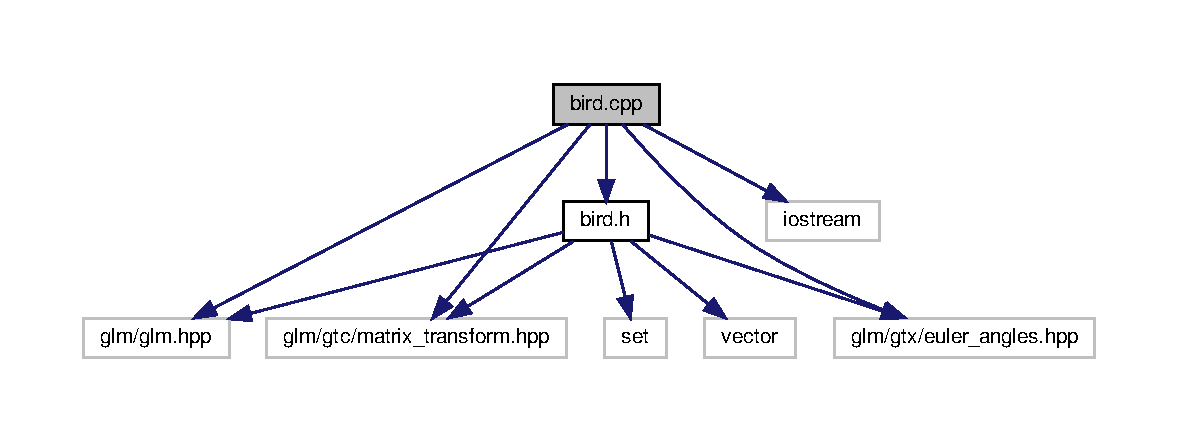
\includegraphics[width=350pt]{bird_8cpp__incl}
\end{center}
\end{figure}

\hypertarget{bird_8h}{}\section{bird.\+h File Reference}
\label{bird_8h}\index{bird.\+h@{bird.\+h}}
{\ttfamily \#include $<$glm/glm.\+hpp$>$}\newline
{\ttfamily \#include $<$glm/gtc/matrix\+\_\+transform.\+hpp$>$}\newline
{\ttfamily \#include $<$glm/gtx/euler\+\_\+angles.\+hpp$>$}\newline
{\ttfamily \#include $<$vector$>$}\newline
{\ttfamily \#include $<$set$>$}\newline
Include dependency graph for bird.\+h\+:
\nopagebreak
\begin{figure}[H]
\begin{center}
\leavevmode
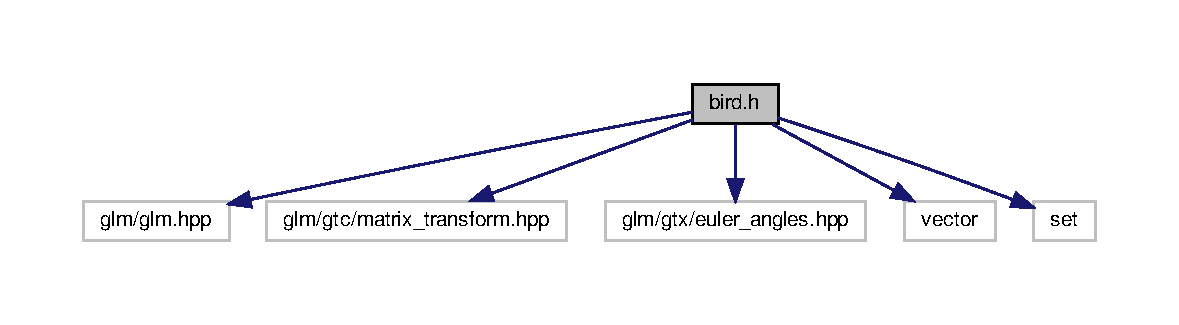
\includegraphics[width=350pt]{bird_8h__incl}
\end{center}
\end{figure}
This graph shows which files directly or indirectly include this file\+:
\nopagebreak
\begin{figure}[H]
\begin{center}
\leavevmode
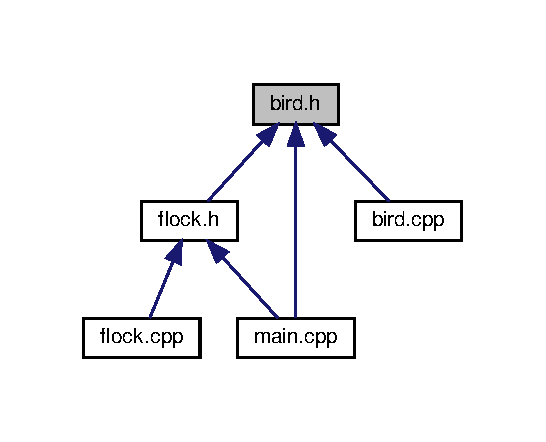
\includegraphics[width=262pt]{bird_8h__dep__incl}
\end{center}
\end{figure}
\subsection*{Classes}
\begin{DoxyCompactItemize}
\item 
class \hyperlink{classBird}{Bird}
\item 
struct \hyperlink{structBird_1_1compare}{Bird\+::compare}
\end{DoxyCompactItemize}
\subsection*{Macros}
\begin{DoxyCompactItemize}
\item 
\#define \hyperlink{bird_8h_a8084e6935f90815089e3fa5038501014}{S\+E\+P\+A\+R\+A\+T\+I\+O\+N\+\_\+\+W\+E\+I\+G\+HT}~0.\+003
\item 
\#define \hyperlink{bird_8h_af64842e7cabadd288bce2516e6fc1683}{A\+L\+I\+G\+M\+E\+N\+T\+\_\+\+W\+E\+I\+G\+HT}~.\+7
\item 
\#define \hyperlink{bird_8h_a290530687e18dcb6fb1be75f4c352045}{C\+O\+H\+E\+S\+I\+O\+N\+\_\+\+W\+E\+I\+G\+HT}~.\+3
\item 
\#define \hyperlink{bird_8h_a5bcb81a070c6570fff9d491fce44f182}{T\+A\+R\+G\+E\+T\+\_\+\+W\+E\+I\+G\+HT}~.\+3
\item 
\#define \hyperlink{bird_8h_ac1f7a2d604fc7bd5501c6ffd4640f1e2}{N\+E\+I\+G\+H\+B\+O\+U\+R\+\_\+\+R\+A\+D\+I\+US}~30.\+8
\item 
\#define \hyperlink{bird_8h_a962c28b54c7841111c4a656056c6a6ee}{D\+E\+S\+I\+R\+E\+D\+\_\+\+S\+E\+P\+A\+R\+A\+T\+I\+ON}~0.\+3
\item 
\#define \hyperlink{bird_8h_ac2cd96d53dd3ba6407db6766c3d92b26}{M\+A\+X\+\_\+\+S\+P\+E\+ED}~0.\+002
\end{DoxyCompactItemize}


\subsection{Macro Definition Documentation}
\mbox{\Hypertarget{bird_8h_af64842e7cabadd288bce2516e6fc1683}\label{bird_8h_af64842e7cabadd288bce2516e6fc1683}} 
\index{bird.\+h@{bird.\+h}!A\+L\+I\+G\+M\+E\+N\+T\+\_\+\+W\+E\+I\+G\+HT@{A\+L\+I\+G\+M\+E\+N\+T\+\_\+\+W\+E\+I\+G\+HT}}
\index{A\+L\+I\+G\+M\+E\+N\+T\+\_\+\+W\+E\+I\+G\+HT@{A\+L\+I\+G\+M\+E\+N\+T\+\_\+\+W\+E\+I\+G\+HT}!bird.\+h@{bird.\+h}}
\subsubsection{\texorpdfstring{A\+L\+I\+G\+M\+E\+N\+T\+\_\+\+W\+E\+I\+G\+HT}{ALIGMENT\_WEIGHT}}
{\footnotesize\ttfamily \#define A\+L\+I\+G\+M\+E\+N\+T\+\_\+\+W\+E\+I\+G\+HT~.\+7}

\mbox{\Hypertarget{bird_8h_a290530687e18dcb6fb1be75f4c352045}\label{bird_8h_a290530687e18dcb6fb1be75f4c352045}} 
\index{bird.\+h@{bird.\+h}!C\+O\+H\+E\+S\+I\+O\+N\+\_\+\+W\+E\+I\+G\+HT@{C\+O\+H\+E\+S\+I\+O\+N\+\_\+\+W\+E\+I\+G\+HT}}
\index{C\+O\+H\+E\+S\+I\+O\+N\+\_\+\+W\+E\+I\+G\+HT@{C\+O\+H\+E\+S\+I\+O\+N\+\_\+\+W\+E\+I\+G\+HT}!bird.\+h@{bird.\+h}}
\subsubsection{\texorpdfstring{C\+O\+H\+E\+S\+I\+O\+N\+\_\+\+W\+E\+I\+G\+HT}{COHESION\_WEIGHT}}
{\footnotesize\ttfamily \#define C\+O\+H\+E\+S\+I\+O\+N\+\_\+\+W\+E\+I\+G\+HT~.\+3}

\mbox{\Hypertarget{bird_8h_a962c28b54c7841111c4a656056c6a6ee}\label{bird_8h_a962c28b54c7841111c4a656056c6a6ee}} 
\index{bird.\+h@{bird.\+h}!D\+E\+S\+I\+R\+E\+D\+\_\+\+S\+E\+P\+A\+R\+A\+T\+I\+ON@{D\+E\+S\+I\+R\+E\+D\+\_\+\+S\+E\+P\+A\+R\+A\+T\+I\+ON}}
\index{D\+E\+S\+I\+R\+E\+D\+\_\+\+S\+E\+P\+A\+R\+A\+T\+I\+ON@{D\+E\+S\+I\+R\+E\+D\+\_\+\+S\+E\+P\+A\+R\+A\+T\+I\+ON}!bird.\+h@{bird.\+h}}
\subsubsection{\texorpdfstring{D\+E\+S\+I\+R\+E\+D\+\_\+\+S\+E\+P\+A\+R\+A\+T\+I\+ON}{DESIRED\_SEPARATION}}
{\footnotesize\ttfamily \#define D\+E\+S\+I\+R\+E\+D\+\_\+\+S\+E\+P\+A\+R\+A\+T\+I\+ON~0.\+3}

\mbox{\Hypertarget{bird_8h_ac2cd96d53dd3ba6407db6766c3d92b26}\label{bird_8h_ac2cd96d53dd3ba6407db6766c3d92b26}} 
\index{bird.\+h@{bird.\+h}!M\+A\+X\+\_\+\+S\+P\+E\+ED@{M\+A\+X\+\_\+\+S\+P\+E\+ED}}
\index{M\+A\+X\+\_\+\+S\+P\+E\+ED@{M\+A\+X\+\_\+\+S\+P\+E\+ED}!bird.\+h@{bird.\+h}}
\subsubsection{\texorpdfstring{M\+A\+X\+\_\+\+S\+P\+E\+ED}{MAX\_SPEED}}
{\footnotesize\ttfamily \#define M\+A\+X\+\_\+\+S\+P\+E\+ED~0.\+002}

\mbox{\Hypertarget{bird_8h_ac1f7a2d604fc7bd5501c6ffd4640f1e2}\label{bird_8h_ac1f7a2d604fc7bd5501c6ffd4640f1e2}} 
\index{bird.\+h@{bird.\+h}!N\+E\+I\+G\+H\+B\+O\+U\+R\+\_\+\+R\+A\+D\+I\+US@{N\+E\+I\+G\+H\+B\+O\+U\+R\+\_\+\+R\+A\+D\+I\+US}}
\index{N\+E\+I\+G\+H\+B\+O\+U\+R\+\_\+\+R\+A\+D\+I\+US@{N\+E\+I\+G\+H\+B\+O\+U\+R\+\_\+\+R\+A\+D\+I\+US}!bird.\+h@{bird.\+h}}
\subsubsection{\texorpdfstring{N\+E\+I\+G\+H\+B\+O\+U\+R\+\_\+\+R\+A\+D\+I\+US}{NEIGHBOUR\_RADIUS}}
{\footnotesize\ttfamily \#define N\+E\+I\+G\+H\+B\+O\+U\+R\+\_\+\+R\+A\+D\+I\+US~30.\+8}

\mbox{\Hypertarget{bird_8h_a8084e6935f90815089e3fa5038501014}\label{bird_8h_a8084e6935f90815089e3fa5038501014}} 
\index{bird.\+h@{bird.\+h}!S\+E\+P\+A\+R\+A\+T\+I\+O\+N\+\_\+\+W\+E\+I\+G\+HT@{S\+E\+P\+A\+R\+A\+T\+I\+O\+N\+\_\+\+W\+E\+I\+G\+HT}}
\index{S\+E\+P\+A\+R\+A\+T\+I\+O\+N\+\_\+\+W\+E\+I\+G\+HT@{S\+E\+P\+A\+R\+A\+T\+I\+O\+N\+\_\+\+W\+E\+I\+G\+HT}!bird.\+h@{bird.\+h}}
\subsubsection{\texorpdfstring{S\+E\+P\+A\+R\+A\+T\+I\+O\+N\+\_\+\+W\+E\+I\+G\+HT}{SEPARATION\_WEIGHT}}
{\footnotesize\ttfamily \#define S\+E\+P\+A\+R\+A\+T\+I\+O\+N\+\_\+\+W\+E\+I\+G\+HT~0.\+003}

\mbox{\Hypertarget{bird_8h_a5bcb81a070c6570fff9d491fce44f182}\label{bird_8h_a5bcb81a070c6570fff9d491fce44f182}} 
\index{bird.\+h@{bird.\+h}!T\+A\+R\+G\+E\+T\+\_\+\+W\+E\+I\+G\+HT@{T\+A\+R\+G\+E\+T\+\_\+\+W\+E\+I\+G\+HT}}
\index{T\+A\+R\+G\+E\+T\+\_\+\+W\+E\+I\+G\+HT@{T\+A\+R\+G\+E\+T\+\_\+\+W\+E\+I\+G\+HT}!bird.\+h@{bird.\+h}}
\subsubsection{\texorpdfstring{T\+A\+R\+G\+E\+T\+\_\+\+W\+E\+I\+G\+HT}{TARGET\_WEIGHT}}
{\footnotesize\ttfamily \#define T\+A\+R\+G\+E\+T\+\_\+\+W\+E\+I\+G\+HT~.\+3}


\hypertarget{flock_8cpp}{}\section{flock.\+cpp File Reference}
\label{flock_8cpp}\index{flock.\+cpp@{flock.\+cpp}}
{\ttfamily \#include \char`\"{}flock.\+h\char`\"{}}\newline
{\ttfamily \#include $<$glm/glm.\+hpp$>$}\newline
{\ttfamily \#include $<$glm/gtc/matrix\+\_\+transform.\+hpp$>$}\newline
{\ttfamily \#include $<$glm/gtx/euler\+\_\+angles.\+hpp$>$}\newline
{\ttfamily \#include \char`\"{}Octree.\+h\char`\"{}}\newline
{\ttfamily \#include $<$iostream$>$}\newline
Include dependency graph for flock.\+cpp\+:
\nopagebreak
\begin{figure}[H]
\begin{center}
\leavevmode
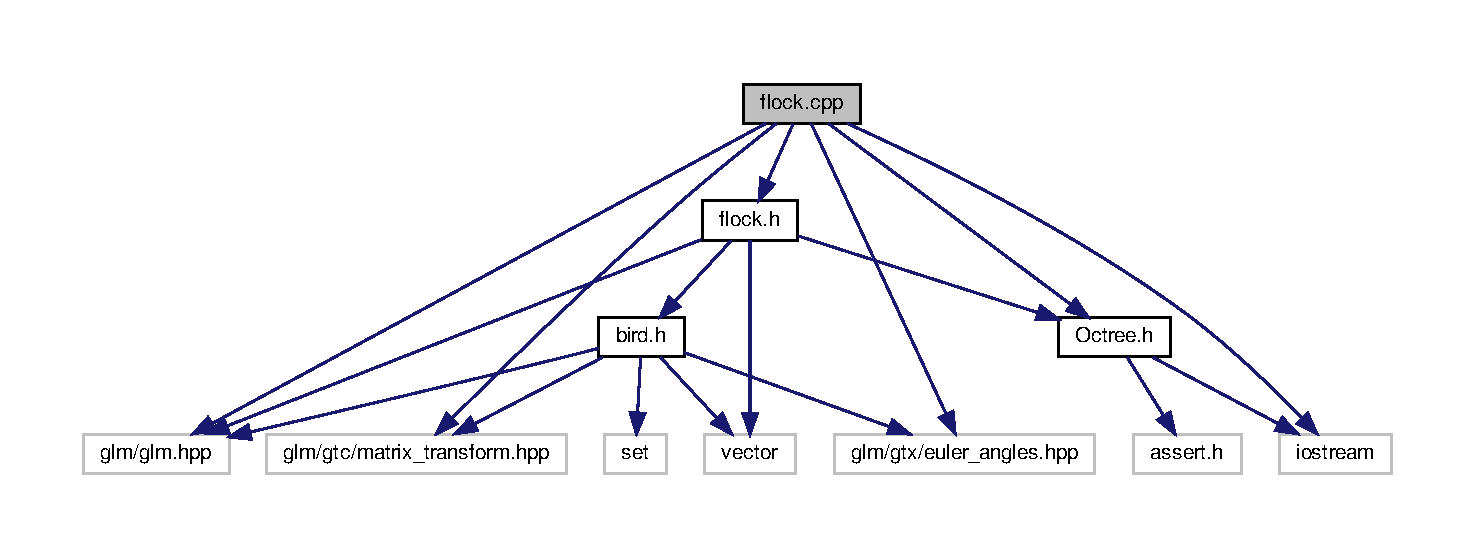
\includegraphics[width=350pt]{flock_8cpp__incl}
\end{center}
\end{figure}

\hypertarget{flock_8h}{}\section{flock.\+h File Reference}
\label{flock_8h}\index{flock.\+h@{flock.\+h}}
{\ttfamily \#include \char`\"{}bird.\+h\char`\"{}}\newline
{\ttfamily \#include \char`\"{}Octree.\+h\char`\"{}}\newline
{\ttfamily \#include $<$glm/glm.\+hpp$>$}\newline
{\ttfamily \#include $<$vector$>$}\newline
Include dependency graph for flock.\+h\+:
\nopagebreak
\begin{figure}[H]
\begin{center}
\leavevmode
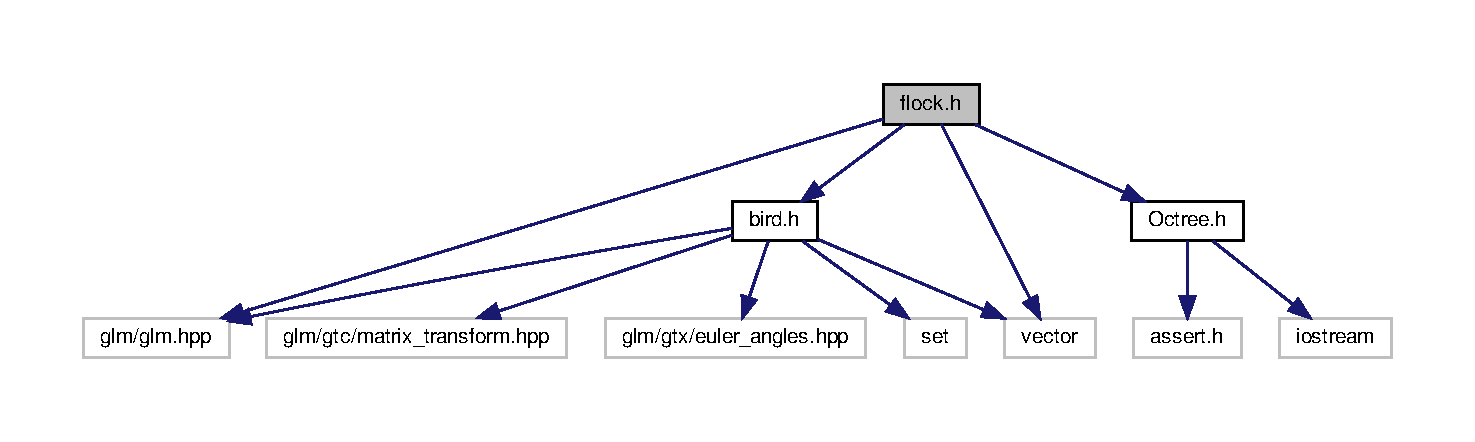
\includegraphics[width=350pt]{flock_8h__incl}
\end{center}
\end{figure}
This graph shows which files directly or indirectly include this file\+:
\nopagebreak
\begin{figure}[H]
\begin{center}
\leavevmode
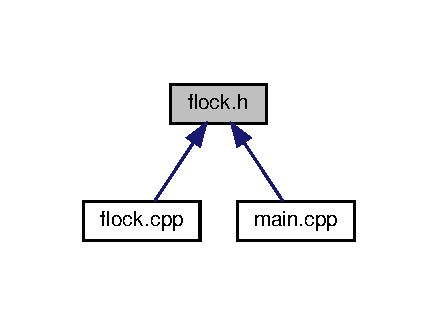
\includegraphics[width=210pt]{flock_8h__dep__incl}
\end{center}
\end{figure}
\subsection*{Classes}
\begin{DoxyCompactItemize}
\item 
struct \hyperlink{structNode}{Node}
\item 
class \hyperlink{classFlock}{Flock}
\end{DoxyCompactItemize}
\subsection*{Macros}
\begin{DoxyCompactItemize}
\item 
\#define \hyperlink{flock_8h_a002b2f4894492820fe708b1b7e7c5e70}{E\+P\+S\+I\+L\+ON}~0.\+0001f
\end{DoxyCompactItemize}


\subsection{Macro Definition Documentation}
\mbox{\Hypertarget{flock_8h_a002b2f4894492820fe708b1b7e7c5e70}\label{flock_8h_a002b2f4894492820fe708b1b7e7c5e70}} 
\index{flock.\+h@{flock.\+h}!E\+P\+S\+I\+L\+ON@{E\+P\+S\+I\+L\+ON}}
\index{E\+P\+S\+I\+L\+ON@{E\+P\+S\+I\+L\+ON}!flock.\+h@{flock.\+h}}
\subsubsection{\texorpdfstring{E\+P\+S\+I\+L\+ON}{EPSILON}}
{\footnotesize\ttfamily \#define E\+P\+S\+I\+L\+ON~0.\+0001f}


\hypertarget{main_8cpp}{}\section{main.\+cpp File Reference}
\label{main_8cpp}\index{main.\+cpp@{main.\+cpp}}
{\ttfamily \#include $<$stdio.\+h$>$}\newline
{\ttfamily \#include $<$stdlib.\+h$>$}\newline
{\ttfamily \#include $<$iostream$>$}\newline
{\ttfamily \#include $<$future$>$}\newline
{\ttfamily \#include $<$vector$>$}\newline
{\ttfamily \#include $<$G\+L/glew.\+h$>$}\newline
{\ttfamily \#include $<$G\+L\+F\+W/glfw3.\+h$>$}\newline
{\ttfamily \#include $<$glm/glm.\+hpp$>$}\newline
{\ttfamily \#include $<$glm/gtc/matrix\+\_\+transform.\+hpp$>$}\newline
{\ttfamily \#include $<$glm/gtx/transform.\+hpp$>$}\newline
{\ttfamily \#include $<$glm/gtx/euler\+\_\+angles.\+hpp$>$}\newline
{\ttfamily \#include $<$glm/gtx/rotate\+\_\+vector.\+hpp$>$}\newline
{\ttfamily \#include $<$G\+L/glut.\+h$>$}\newline
{\ttfamily \#include $<$shader.\+hpp$>$}\newline
{\ttfamily \#include $<$texture.\+hpp$>$}\newline
{\ttfamily \#include $<$flock.\+h$>$}\newline
{\ttfamily \#include $<$bird.\+h$>$}\newline
{\ttfamily \#include $<$simul\+Timer.\+h$>$}\newline
{\ttfamily \#include $<$objloader.\+hpp$>$}\newline
{\ttfamily \#include $<$math.\+h$>$}\newline
{\ttfamily \#include \char`\"{}glm/gtx/string\+\_\+cast.\+hpp\char`\"{}}\newline
Include dependency graph for main.\+cpp\+:
\nopagebreak
\begin{figure}[H]
\begin{center}
\leavevmode
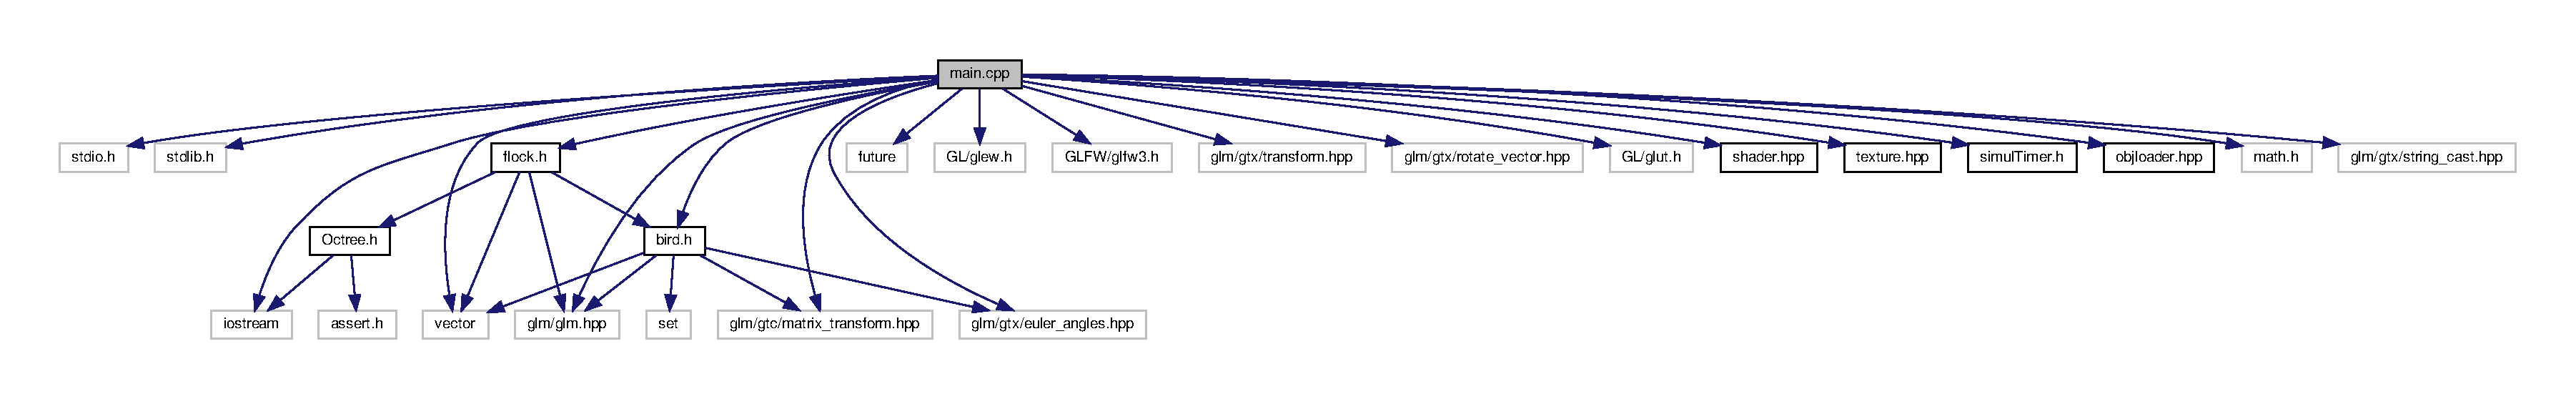
\includegraphics[width=350pt]{main_8cpp__incl}
\end{center}
\end{figure}
\subsection*{Macros}
\begin{DoxyCompactItemize}
\item 
\#define \hyperlink{main_8cpp_a598a3330b3c21701223ee0ca14316eca}{PI}~3.\+14f
\item 
\#define \hyperlink{main_8cpp_a85f21588f69ad91603849de447868fc1}{F\+L\+O\+C\+K\+\_\+\+S\+I\+ZE}~100
\item 
\#define \hyperlink{main_8cpp_ab39fec97d85960796efedec442f38004}{I\+N\+T\+E\+R\+V\+AL}~3500
\end{DoxyCompactItemize}
\subsection*{Functions}
\begin{DoxyCompactItemize}
\item 
void \hyperlink{main_8cpp_a5382c76c0c292c76ddca426e79ad53ba}{render\+Boid} (vec3 pos, vec3 velocity)
\item 
void \hyperlink{main_8cpp_ae357309218a54bd5e4b1b7384aad7d43}{render\+Flock} (std\+::vector$<$ vec3 $>$ positions, std\+::vector$<$ vec3 $>$ velocities)
\item 
void \hyperlink{main_8cpp_a47bc1e4f1c5cd638d0d874656b5e42c5}{update\+Flock} (\hyperlink{classFlock}{Flock} flock)
\item 
int \hyperlink{main_8cpp_a840291bc02cba5474a4cb46a9b9566fe}{main} (void)
\item 
void \hyperlink{main_8cpp_ad5d35421be86f18ae8124f285be25b7a}{mouse\+Call\+Back} ()
\item 
void \hyperlink{main_8cpp_af862c2d9fec42d60d8397eaba2b438ed}{motion\+Call\+Back} ()
\item 
void \hyperlink{main_8cpp_a64c582abc11d1b9939c4a03036188a41}{display\+Func} ()
\end{DoxyCompactItemize}
\subsection*{Variables}
\begin{DoxyCompactItemize}
\item 
G\+L\+F\+Wwindow $\ast$ \hyperlink{main_8cpp_a80de27bd7dc4e2b2ad3d5895b97a70f0}{window}
\item 
float \hyperlink{main_8cpp_a3d47f7e2bf80c3044a1c4fb985d08565}{separation} = 0.\+003f
\item 
float \hyperlink{main_8cpp_a9b609437b0a9c5266747f6a31b8bf90e}{alignment} = 0.\+7f
\item 
float \hyperlink{main_8cpp_ab665ec90cc49c91ed2d1e7e0ca3c386e}{cohesion} = 0.\+3f
\item 
float \hyperlink{main_8cpp_af0df2177301e4061ab72ade2ea437bcd}{target} = 0.\+3f
\item 
bool \hyperlink{main_8cpp_aae9e26fee26af7722250e6b27dbdf37a}{target\+\_\+present} =true
\item 
G\+Luint \hyperlink{main_8cpp_a391fd187e1c163e1bc7dc26a34c402f2}{program\+ID}
\item 
G\+Luint \hyperlink{main_8cpp_a6f91d732d0b524c77be0df6beaa6d55f}{Matrix\+ID}
\item 
G\+Luint \hyperlink{main_8cpp_ab19cf36286363450e9a1a48f906f606f}{View\+Matrix\+ID}
\item 
G\+Luint \hyperlink{main_8cpp_ad471614cd302ae9dcc9f95cbb8d9e8fc}{Model\+Matrix\+ID}
\item 
std\+::vector$<$ glm\+::vec3 $>$ \hyperlink{main_8cpp_afbb9924ed1034bf20e5bf8b38f066567}{vertices}
\item 
glm\+::mat4 \hyperlink{main_8cpp_ab276b213c71fd372d962f617566518be}{View\+Matrix}
\item 
glm\+::mat4 \hyperlink{main_8cpp_af437a7042c55c02cfdbd4a1e074b890a}{Projection\+Matrix}
\item 
glm\+::mat4 \hyperlink{main_8cpp_a9bf91bc5771e47fdb3c7261ca19a3155}{M\+VP}
\item 
glm\+::mat4 \hyperlink{main_8cpp_a69296e88c57209be1d9dfea383abcc0d}{Model\+Matrix}
\item 
glm\+::mat4 \hyperlink{main_8cpp_a386c5cb6b9262f694155a0fe1c3b59c8}{Scaling\+Matrix}
\item 
glm\+::mat4 \hyperlink{main_8cpp_a7cb1d8950469897786959fc93eac4652}{Translation\+Matrix}
\item 
glm\+::mat4 \hyperlink{main_8cpp_ae1481fbae22ad889b3048ce68edf6ec8}{Rotation\+Matrix}
\end{DoxyCompactItemize}


\subsection{Macro Definition Documentation}
\mbox{\Hypertarget{main_8cpp_a85f21588f69ad91603849de447868fc1}\label{main_8cpp_a85f21588f69ad91603849de447868fc1}} 
\index{main.\+cpp@{main.\+cpp}!F\+L\+O\+C\+K\+\_\+\+S\+I\+ZE@{F\+L\+O\+C\+K\+\_\+\+S\+I\+ZE}}
\index{F\+L\+O\+C\+K\+\_\+\+S\+I\+ZE@{F\+L\+O\+C\+K\+\_\+\+S\+I\+ZE}!main.\+cpp@{main.\+cpp}}
\subsubsection{\texorpdfstring{F\+L\+O\+C\+K\+\_\+\+S\+I\+ZE}{FLOCK\_SIZE}}
{\footnotesize\ttfamily \#define F\+L\+O\+C\+K\+\_\+\+S\+I\+ZE~100}

\mbox{\Hypertarget{main_8cpp_ab39fec97d85960796efedec442f38004}\label{main_8cpp_ab39fec97d85960796efedec442f38004}} 
\index{main.\+cpp@{main.\+cpp}!I\+N\+T\+E\+R\+V\+AL@{I\+N\+T\+E\+R\+V\+AL}}
\index{I\+N\+T\+E\+R\+V\+AL@{I\+N\+T\+E\+R\+V\+AL}!main.\+cpp@{main.\+cpp}}
\subsubsection{\texorpdfstring{I\+N\+T\+E\+R\+V\+AL}{INTERVAL}}
{\footnotesize\ttfamily \#define I\+N\+T\+E\+R\+V\+AL~3500}

\mbox{\Hypertarget{main_8cpp_a598a3330b3c21701223ee0ca14316eca}\label{main_8cpp_a598a3330b3c21701223ee0ca14316eca}} 
\index{main.\+cpp@{main.\+cpp}!PI@{PI}}
\index{PI@{PI}!main.\+cpp@{main.\+cpp}}
\subsubsection{\texorpdfstring{PI}{PI}}
{\footnotesize\ttfamily \#define PI~3.\+14f}



\subsection{Function Documentation}
\mbox{\Hypertarget{main_8cpp_a64c582abc11d1b9939c4a03036188a41}\label{main_8cpp_a64c582abc11d1b9939c4a03036188a41}} 
\index{main.\+cpp@{main.\+cpp}!display\+Func@{display\+Func}}
\index{display\+Func@{display\+Func}!main.\+cpp@{main.\+cpp}}
\subsubsection{\texorpdfstring{display\+Func()}{displayFunc()}}
{\footnotesize\ttfamily void display\+Func (\begin{DoxyParamCaption}{ }\end{DoxyParamCaption})}

\mbox{\Hypertarget{main_8cpp_a840291bc02cba5474a4cb46a9b9566fe}\label{main_8cpp_a840291bc02cba5474a4cb46a9b9566fe}} 
\index{main.\+cpp@{main.\+cpp}!main@{main}}
\index{main@{main}!main.\+cpp@{main.\+cpp}}
\subsubsection{\texorpdfstring{main()}{main()}}
{\footnotesize\ttfamily int main (\begin{DoxyParamCaption}\item[{void}]{ }\end{DoxyParamCaption})}

\mbox{\Hypertarget{main_8cpp_af862c2d9fec42d60d8397eaba2b438ed}\label{main_8cpp_af862c2d9fec42d60d8397eaba2b438ed}} 
\index{main.\+cpp@{main.\+cpp}!motion\+Call\+Back@{motion\+Call\+Back}}
\index{motion\+Call\+Back@{motion\+Call\+Back}!main.\+cpp@{main.\+cpp}}
\subsubsection{\texorpdfstring{motion\+Call\+Back()}{motionCallBack()}}
{\footnotesize\ttfamily void motion\+Call\+Back (\begin{DoxyParamCaption}{ }\end{DoxyParamCaption})}

\mbox{\Hypertarget{main_8cpp_ad5d35421be86f18ae8124f285be25b7a}\label{main_8cpp_ad5d35421be86f18ae8124f285be25b7a}} 
\index{main.\+cpp@{main.\+cpp}!mouse\+Call\+Back@{mouse\+Call\+Back}}
\index{mouse\+Call\+Back@{mouse\+Call\+Back}!main.\+cpp@{main.\+cpp}}
\subsubsection{\texorpdfstring{mouse\+Call\+Back()}{mouseCallBack()}}
{\footnotesize\ttfamily void mouse\+Call\+Back (\begin{DoxyParamCaption}{ }\end{DoxyParamCaption})}

\mbox{\Hypertarget{main_8cpp_a5382c76c0c292c76ddca426e79ad53ba}\label{main_8cpp_a5382c76c0c292c76ddca426e79ad53ba}} 
\index{main.\+cpp@{main.\+cpp}!render\+Boid@{render\+Boid}}
\index{render\+Boid@{render\+Boid}!main.\+cpp@{main.\+cpp}}
\subsubsection{\texorpdfstring{render\+Boid()}{renderBoid()}}
{\footnotesize\ttfamily void render\+Boid (\begin{DoxyParamCaption}\item[{vec3}]{pos,  }\item[{vec3}]{velocity }\end{DoxyParamCaption})}

\mbox{\Hypertarget{main_8cpp_ae357309218a54bd5e4b1b7384aad7d43}\label{main_8cpp_ae357309218a54bd5e4b1b7384aad7d43}} 
\index{main.\+cpp@{main.\+cpp}!render\+Flock@{render\+Flock}}
\index{render\+Flock@{render\+Flock}!main.\+cpp@{main.\+cpp}}
\subsubsection{\texorpdfstring{render\+Flock()}{renderFlock()}}
{\footnotesize\ttfamily void render\+Flock (\begin{DoxyParamCaption}\item[{std\+::vector$<$ vec3 $>$}]{positions,  }\item[{std\+::vector$<$ vec3 $>$}]{velocities }\end{DoxyParamCaption})}

\mbox{\Hypertarget{main_8cpp_a47bc1e4f1c5cd638d0d874656b5e42c5}\label{main_8cpp_a47bc1e4f1c5cd638d0d874656b5e42c5}} 
\index{main.\+cpp@{main.\+cpp}!update\+Flock@{update\+Flock}}
\index{update\+Flock@{update\+Flock}!main.\+cpp@{main.\+cpp}}
\subsubsection{\texorpdfstring{update\+Flock()}{updateFlock()}}
{\footnotesize\ttfamily void update\+Flock (\begin{DoxyParamCaption}\item[{\hyperlink{classFlock}{Flock}}]{flock }\end{DoxyParamCaption})}



\subsection{Variable Documentation}
\mbox{\Hypertarget{main_8cpp_a9b609437b0a9c5266747f6a31b8bf90e}\label{main_8cpp_a9b609437b0a9c5266747f6a31b8bf90e}} 
\index{main.\+cpp@{main.\+cpp}!alignment@{alignment}}
\index{alignment@{alignment}!main.\+cpp@{main.\+cpp}}
\subsubsection{\texorpdfstring{alignment}{alignment}}
{\footnotesize\ttfamily float alignment = 0.\+7f}

\mbox{\Hypertarget{main_8cpp_ab665ec90cc49c91ed2d1e7e0ca3c386e}\label{main_8cpp_ab665ec90cc49c91ed2d1e7e0ca3c386e}} 
\index{main.\+cpp@{main.\+cpp}!cohesion@{cohesion}}
\index{cohesion@{cohesion}!main.\+cpp@{main.\+cpp}}
\subsubsection{\texorpdfstring{cohesion}{cohesion}}
{\footnotesize\ttfamily float cohesion = 0.\+3f}

\mbox{\Hypertarget{main_8cpp_a6f91d732d0b524c77be0df6beaa6d55f}\label{main_8cpp_a6f91d732d0b524c77be0df6beaa6d55f}} 
\index{main.\+cpp@{main.\+cpp}!Matrix\+ID@{Matrix\+ID}}
\index{Matrix\+ID@{Matrix\+ID}!main.\+cpp@{main.\+cpp}}
\subsubsection{\texorpdfstring{Matrix\+ID}{MatrixID}}
{\footnotesize\ttfamily G\+Luint Matrix\+ID}

\mbox{\Hypertarget{main_8cpp_a69296e88c57209be1d9dfea383abcc0d}\label{main_8cpp_a69296e88c57209be1d9dfea383abcc0d}} 
\index{main.\+cpp@{main.\+cpp}!Model\+Matrix@{Model\+Matrix}}
\index{Model\+Matrix@{Model\+Matrix}!main.\+cpp@{main.\+cpp}}
\subsubsection{\texorpdfstring{Model\+Matrix}{ModelMatrix}}
{\footnotesize\ttfamily glm\+::mat4 Model\+Matrix}

\mbox{\Hypertarget{main_8cpp_ad471614cd302ae9dcc9f95cbb8d9e8fc}\label{main_8cpp_ad471614cd302ae9dcc9f95cbb8d9e8fc}} 
\index{main.\+cpp@{main.\+cpp}!Model\+Matrix\+ID@{Model\+Matrix\+ID}}
\index{Model\+Matrix\+ID@{Model\+Matrix\+ID}!main.\+cpp@{main.\+cpp}}
\subsubsection{\texorpdfstring{Model\+Matrix\+ID}{ModelMatrixID}}
{\footnotesize\ttfamily G\+Luint Model\+Matrix\+ID}

\mbox{\Hypertarget{main_8cpp_a9bf91bc5771e47fdb3c7261ca19a3155}\label{main_8cpp_a9bf91bc5771e47fdb3c7261ca19a3155}} 
\index{main.\+cpp@{main.\+cpp}!M\+VP@{M\+VP}}
\index{M\+VP@{M\+VP}!main.\+cpp@{main.\+cpp}}
\subsubsection{\texorpdfstring{M\+VP}{MVP}}
{\footnotesize\ttfamily glm\+::mat4 M\+VP}

\mbox{\Hypertarget{main_8cpp_a391fd187e1c163e1bc7dc26a34c402f2}\label{main_8cpp_a391fd187e1c163e1bc7dc26a34c402f2}} 
\index{main.\+cpp@{main.\+cpp}!program\+ID@{program\+ID}}
\index{program\+ID@{program\+ID}!main.\+cpp@{main.\+cpp}}
\subsubsection{\texorpdfstring{program\+ID}{programID}}
{\footnotesize\ttfamily G\+Luint program\+ID}

\mbox{\Hypertarget{main_8cpp_af437a7042c55c02cfdbd4a1e074b890a}\label{main_8cpp_af437a7042c55c02cfdbd4a1e074b890a}} 
\index{main.\+cpp@{main.\+cpp}!Projection\+Matrix@{Projection\+Matrix}}
\index{Projection\+Matrix@{Projection\+Matrix}!main.\+cpp@{main.\+cpp}}
\subsubsection{\texorpdfstring{Projection\+Matrix}{ProjectionMatrix}}
{\footnotesize\ttfamily glm\+::mat4 Projection\+Matrix}

\mbox{\Hypertarget{main_8cpp_ae1481fbae22ad889b3048ce68edf6ec8}\label{main_8cpp_ae1481fbae22ad889b3048ce68edf6ec8}} 
\index{main.\+cpp@{main.\+cpp}!Rotation\+Matrix@{Rotation\+Matrix}}
\index{Rotation\+Matrix@{Rotation\+Matrix}!main.\+cpp@{main.\+cpp}}
\subsubsection{\texorpdfstring{Rotation\+Matrix}{RotationMatrix}}
{\footnotesize\ttfamily glm\+::mat4 Rotation\+Matrix}

\mbox{\Hypertarget{main_8cpp_a386c5cb6b9262f694155a0fe1c3b59c8}\label{main_8cpp_a386c5cb6b9262f694155a0fe1c3b59c8}} 
\index{main.\+cpp@{main.\+cpp}!Scaling\+Matrix@{Scaling\+Matrix}}
\index{Scaling\+Matrix@{Scaling\+Matrix}!main.\+cpp@{main.\+cpp}}
\subsubsection{\texorpdfstring{Scaling\+Matrix}{ScalingMatrix}}
{\footnotesize\ttfamily glm\+::mat4 Scaling\+Matrix}

\mbox{\Hypertarget{main_8cpp_a3d47f7e2bf80c3044a1c4fb985d08565}\label{main_8cpp_a3d47f7e2bf80c3044a1c4fb985d08565}} 
\index{main.\+cpp@{main.\+cpp}!separation@{separation}}
\index{separation@{separation}!main.\+cpp@{main.\+cpp}}
\subsubsection{\texorpdfstring{separation}{separation}}
{\footnotesize\ttfamily float separation = 0.\+003f}

\mbox{\Hypertarget{main_8cpp_af0df2177301e4061ab72ade2ea437bcd}\label{main_8cpp_af0df2177301e4061ab72ade2ea437bcd}} 
\index{main.\+cpp@{main.\+cpp}!target@{target}}
\index{target@{target}!main.\+cpp@{main.\+cpp}}
\subsubsection{\texorpdfstring{target}{target}}
{\footnotesize\ttfamily float target = 0.\+3f}

\mbox{\Hypertarget{main_8cpp_aae9e26fee26af7722250e6b27dbdf37a}\label{main_8cpp_aae9e26fee26af7722250e6b27dbdf37a}} 
\index{main.\+cpp@{main.\+cpp}!target\+\_\+present@{target\+\_\+present}}
\index{target\+\_\+present@{target\+\_\+present}!main.\+cpp@{main.\+cpp}}
\subsubsection{\texorpdfstring{target\+\_\+present}{target\_present}}
{\footnotesize\ttfamily bool target\+\_\+present =true}

\mbox{\Hypertarget{main_8cpp_a7cb1d8950469897786959fc93eac4652}\label{main_8cpp_a7cb1d8950469897786959fc93eac4652}} 
\index{main.\+cpp@{main.\+cpp}!Translation\+Matrix@{Translation\+Matrix}}
\index{Translation\+Matrix@{Translation\+Matrix}!main.\+cpp@{main.\+cpp}}
\subsubsection{\texorpdfstring{Translation\+Matrix}{TranslationMatrix}}
{\footnotesize\ttfamily glm\+::mat4 Translation\+Matrix}

\mbox{\Hypertarget{main_8cpp_afbb9924ed1034bf20e5bf8b38f066567}\label{main_8cpp_afbb9924ed1034bf20e5bf8b38f066567}} 
\index{main.\+cpp@{main.\+cpp}!vertices@{vertices}}
\index{vertices@{vertices}!main.\+cpp@{main.\+cpp}}
\subsubsection{\texorpdfstring{vertices}{vertices}}
{\footnotesize\ttfamily std\+::vector$<$glm\+::vec3$>$ vertices}

\mbox{\Hypertarget{main_8cpp_ab276b213c71fd372d962f617566518be}\label{main_8cpp_ab276b213c71fd372d962f617566518be}} 
\index{main.\+cpp@{main.\+cpp}!View\+Matrix@{View\+Matrix}}
\index{View\+Matrix@{View\+Matrix}!main.\+cpp@{main.\+cpp}}
\subsubsection{\texorpdfstring{View\+Matrix}{ViewMatrix}}
{\footnotesize\ttfamily glm\+::mat4 View\+Matrix}

\mbox{\Hypertarget{main_8cpp_ab19cf36286363450e9a1a48f906f606f}\label{main_8cpp_ab19cf36286363450e9a1a48f906f606f}} 
\index{main.\+cpp@{main.\+cpp}!View\+Matrix\+ID@{View\+Matrix\+ID}}
\index{View\+Matrix\+ID@{View\+Matrix\+ID}!main.\+cpp@{main.\+cpp}}
\subsubsection{\texorpdfstring{View\+Matrix\+ID}{ViewMatrixID}}
{\footnotesize\ttfamily G\+Luint View\+Matrix\+ID}

\mbox{\Hypertarget{main_8cpp_a80de27bd7dc4e2b2ad3d5895b97a70f0}\label{main_8cpp_a80de27bd7dc4e2b2ad3d5895b97a70f0}} 
\index{main.\+cpp@{main.\+cpp}!window@{window}}
\index{window@{window}!main.\+cpp@{main.\+cpp}}
\subsubsection{\texorpdfstring{window}{window}}
{\footnotesize\ttfamily G\+L\+F\+Wwindow$\ast$ window}


\hypertarget{objloader_8cpp}{}\section{objloader.\+cpp File Reference}
\label{objloader_8cpp}\index{objloader.\+cpp@{objloader.\+cpp}}
{\ttfamily \#include $<$vector$>$}\newline
{\ttfamily \#include $<$stdio.\+h$>$}\newline
{\ttfamily \#include $<$string$>$}\newline
{\ttfamily \#include $<$cstring$>$}\newline
{\ttfamily \#include $<$glm/glm.\+hpp$>$}\newline
{\ttfamily \#include \char`\"{}objloader.\+hpp\char`\"{}}\newline
Include dependency graph for objloader.\+cpp\+:
\nopagebreak
\begin{figure}[H]
\begin{center}
\leavevmode
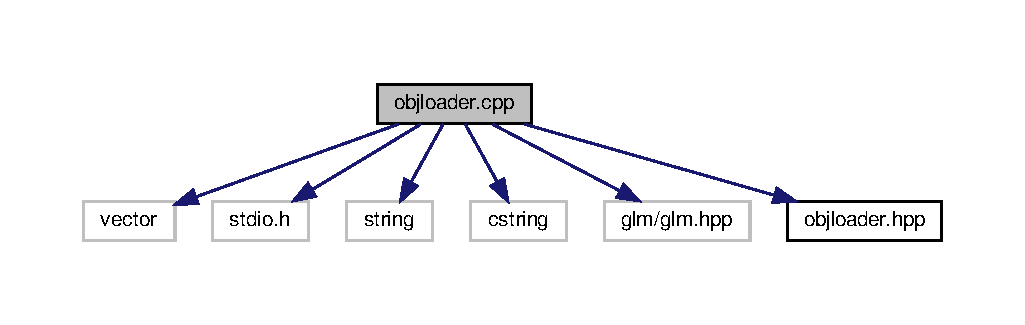
\includegraphics[width=350pt]{objloader_8cpp__incl}
\end{center}
\end{figure}
\subsection*{Functions}
\begin{DoxyCompactItemize}
\item 
bool \hyperlink{objloader_8cpp_a787a44bc3c93cec3fd01c39488b09e08}{load\+O\+BJ} (const char $\ast$path, std\+::vector$<$ glm\+::vec3 $>$ \&out\+\_\+vertices, std\+::vector$<$ glm\+::vec2 $>$ \&out\+\_\+uvs, std\+::vector$<$ glm\+::vec3 $>$ \&out\+\_\+normals)
\end{DoxyCompactItemize}


\subsection{Function Documentation}
\mbox{\Hypertarget{objloader_8cpp_a787a44bc3c93cec3fd01c39488b09e08}\label{objloader_8cpp_a787a44bc3c93cec3fd01c39488b09e08}} 
\index{objloader.\+cpp@{objloader.\+cpp}!load\+O\+BJ@{load\+O\+BJ}}
\index{load\+O\+BJ@{load\+O\+BJ}!objloader.\+cpp@{objloader.\+cpp}}
\subsubsection{\texorpdfstring{load\+O\+B\+J()}{loadOBJ()}}
{\footnotesize\ttfamily bool load\+O\+BJ (\begin{DoxyParamCaption}\item[{const char $\ast$}]{path,  }\item[{std\+::vector$<$ glm\+::vec3 $>$ \&}]{out\+\_\+vertices,  }\item[{std\+::vector$<$ glm\+::vec2 $>$ \&}]{out\+\_\+uvs,  }\item[{std\+::vector$<$ glm\+::vec3 $>$ \&}]{out\+\_\+normals }\end{DoxyParamCaption})}


\hypertarget{objloader_8hpp}{}\section{objloader.\+hpp File Reference}
\label{objloader_8hpp}\index{objloader.\+hpp@{objloader.\+hpp}}
This graph shows which files directly or indirectly include this file\+:
\nopagebreak
\begin{figure}[H]
\begin{center}
\leavevmode
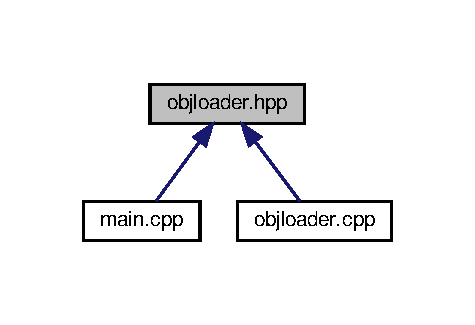
\includegraphics[width=228pt]{objloader_8hpp__dep__incl}
\end{center}
\end{figure}
\subsection*{Functions}
\begin{DoxyCompactItemize}
\item 
bool \hyperlink{objloader_8hpp_a787a44bc3c93cec3fd01c39488b09e08}{load\+O\+BJ} (const char $\ast$path, std\+::vector$<$ glm\+::vec3 $>$ \&out\+\_\+vertices, std\+::vector$<$ glm\+::vec2 $>$ \&out\+\_\+uvs, std\+::vector$<$ glm\+::vec3 $>$ \&out\+\_\+normals)
\item 
bool \hyperlink{objloader_8hpp_a77e6cdf2f11991cec1613baebb0e2785}{load\+Ass\+Imp} (const char $\ast$path, std\+::vector$<$ unsigned short $>$ \&indices, std\+::vector$<$ glm\+::vec3 $>$ \&\hyperlink{main_8cpp_afbb9924ed1034bf20e5bf8b38f066567}{vertices}, std\+::vector$<$ glm\+::vec2 $>$ \&uvs, std\+::vector$<$ glm\+::vec3 $>$ \&normals)
\end{DoxyCompactItemize}


\subsection{Function Documentation}
\mbox{\Hypertarget{objloader_8hpp_a77e6cdf2f11991cec1613baebb0e2785}\label{objloader_8hpp_a77e6cdf2f11991cec1613baebb0e2785}} 
\index{objloader.\+hpp@{objloader.\+hpp}!load\+Ass\+Imp@{load\+Ass\+Imp}}
\index{load\+Ass\+Imp@{load\+Ass\+Imp}!objloader.\+hpp@{objloader.\+hpp}}
\subsubsection{\texorpdfstring{load\+Ass\+Imp()}{loadAssImp()}}
{\footnotesize\ttfamily bool load\+Ass\+Imp (\begin{DoxyParamCaption}\item[{const char $\ast$}]{path,  }\item[{std\+::vector$<$ unsigned short $>$ \&}]{indices,  }\item[{std\+::vector$<$ glm\+::vec3 $>$ \&}]{vertices,  }\item[{std\+::vector$<$ glm\+::vec2 $>$ \&}]{uvs,  }\item[{std\+::vector$<$ glm\+::vec3 $>$ \&}]{normals }\end{DoxyParamCaption})}

\mbox{\Hypertarget{objloader_8hpp_a787a44bc3c93cec3fd01c39488b09e08}\label{objloader_8hpp_a787a44bc3c93cec3fd01c39488b09e08}} 
\index{objloader.\+hpp@{objloader.\+hpp}!load\+O\+BJ@{load\+O\+BJ}}
\index{load\+O\+BJ@{load\+O\+BJ}!objloader.\+hpp@{objloader.\+hpp}}
\subsubsection{\texorpdfstring{load\+O\+B\+J()}{loadOBJ()}}
{\footnotesize\ttfamily bool load\+O\+BJ (\begin{DoxyParamCaption}\item[{const char $\ast$}]{path,  }\item[{std\+::vector$<$ glm\+::vec3 $>$ \&}]{out\+\_\+vertices,  }\item[{std\+::vector$<$ glm\+::vec2 $>$ \&}]{out\+\_\+uvs,  }\item[{std\+::vector$<$ glm\+::vec3 $>$ \&}]{out\+\_\+normals }\end{DoxyParamCaption})}


\hypertarget{Octree_8h}{}\section{Octree.\+h File Reference}
\label{Octree_8h}\index{Octree.\+h@{Octree.\+h}}
{\ttfamily \#include $<$assert.\+h$>$}\newline
{\ttfamily \#include $<$iostream$>$}\newline
Include dependency graph for Octree.\+h\+:
\nopagebreak
\begin{figure}[H]
\begin{center}
\leavevmode
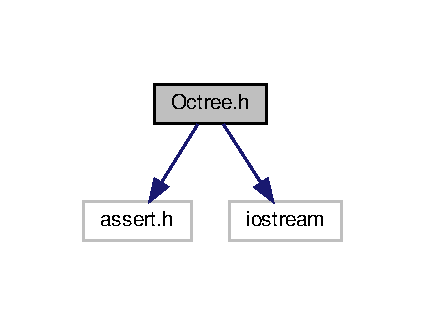
\includegraphics[width=204pt]{Octree_8h__incl}
\end{center}
\end{figure}
This graph shows which files directly or indirectly include this file\+:
\nopagebreak
\begin{figure}[H]
\begin{center}
\leavevmode
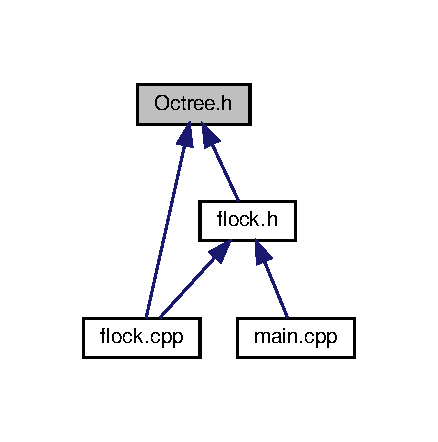
\includegraphics[width=210pt]{Octree_8h__dep__incl}
\end{center}
\end{figure}
\subsection*{Classes}
\begin{DoxyCompactItemize}
\item 
class \hyperlink{classOctree}{Octree$<$ N $>$}
\item 
struct \hyperlink{structOctree_1_1Point}{Octree$<$ N $>$\+::\+Point}
\item 
struct \hyperlink{structOctree_1_1OctreeNode}{Octree$<$ N $>$\+::\+Octree\+Node}
\item 
class \hyperlink{classOctree_1_1Callback}{Octree$<$ N $>$\+::\+Callback}
\item 
class \hyperlink{classOctree_1_1Iterator}{Octree$<$ N $>$\+::\+Iterator}
\end{DoxyCompactItemize}
\subsection*{Macros}
\begin{DoxyCompactItemize}
\item 
\#define \hyperlink{Octree_8h_af5c33ba4be67eaa3d6ff8e2e3db215d2}{C\+O\+M\+P\+U\+T\+E\+\_\+\+S\+I\+DE}(i,  bit,  p,  mid,  new\+Min,  new\+Max)
\end{DoxyCompactItemize}


\subsection{Macro Definition Documentation}
\mbox{\Hypertarget{Octree_8h_af5c33ba4be67eaa3d6ff8e2e3db215d2}\label{Octree_8h_af5c33ba4be67eaa3d6ff8e2e3db215d2}} 
\index{Octree.\+h@{Octree.\+h}!C\+O\+M\+P\+U\+T\+E\+\_\+\+S\+I\+DE@{C\+O\+M\+P\+U\+T\+E\+\_\+\+S\+I\+DE}}
\index{C\+O\+M\+P\+U\+T\+E\+\_\+\+S\+I\+DE@{C\+O\+M\+P\+U\+T\+E\+\_\+\+S\+I\+DE}!Octree.\+h@{Octree.\+h}}
\subsubsection{\texorpdfstring{C\+O\+M\+P\+U\+T\+E\+\_\+\+S\+I\+DE}{COMPUTE\_SIDE}}
{\footnotesize\ttfamily \#define C\+O\+M\+P\+U\+T\+E\+\_\+\+S\+I\+DE(\begin{DoxyParamCaption}\item[{}]{i,  }\item[{}]{bit,  }\item[{}]{p,  }\item[{}]{mid,  }\item[{}]{new\+Min,  }\item[{}]{new\+Max }\end{DoxyParamCaption})}

{\bfseries Value\+:}
\begin{DoxyCode}
\textcolor{keywordflow}{if} (p >= mid)         \(\backslash\)
\{                     \(\backslash\)
    i |= bit;         \(\backslash\)
    newMin = mid;     \(\backslash\)
\}                     \(\backslash\)
else                  \(\backslash\)
\{                     \(\backslash\)
    newMax = mid;     \(\backslash\)
\}
\end{DoxyCode}

\hypertarget{shader_8cpp}{}\section{shader.\+cpp File Reference}
\label{shader_8cpp}\index{shader.\+cpp@{shader.\+cpp}}
{\ttfamily \#include $<$stdio.\+h$>$}\newline
{\ttfamily \#include $<$string$>$}\newline
{\ttfamily \#include $<$vector$>$}\newline
{\ttfamily \#include $<$iostream$>$}\newline
{\ttfamily \#include $<$fstream$>$}\newline
{\ttfamily \#include $<$algorithm$>$}\newline
{\ttfamily \#include $<$sstream$>$}\newline
{\ttfamily \#include $<$stdlib.\+h$>$}\newline
{\ttfamily \#include $<$string.\+h$>$}\newline
{\ttfamily \#include $<$G\+L/glew.\+h$>$}\newline
{\ttfamily \#include \char`\"{}shader.\+hpp\char`\"{}}\newline
Include dependency graph for shader.\+cpp\+:
\nopagebreak
\begin{figure}[H]
\begin{center}
\leavevmode
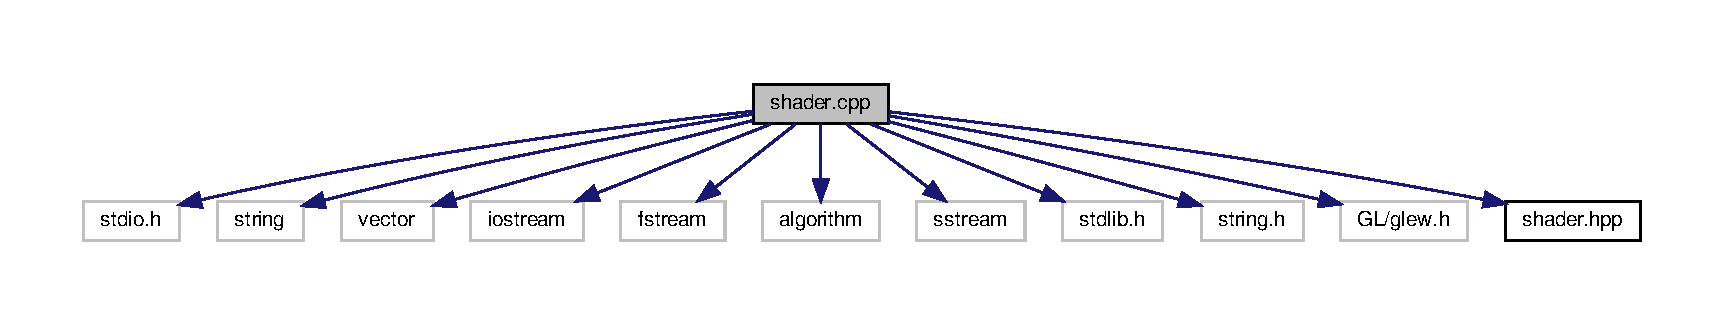
\includegraphics[width=350pt]{shader_8cpp__incl}
\end{center}
\end{figure}
\subsection*{Functions}
\begin{DoxyCompactItemize}
\item 
G\+Luint \hyperlink{shader_8cpp_a833f10cca6a76fe34ae9efa23ac5e73c}{Load\+Shaders} (const char $\ast$vertex\+\_\+file\+\_\+path, const char $\ast$fragment\+\_\+file\+\_\+path)
\end{DoxyCompactItemize}


\subsection{Function Documentation}
\mbox{\Hypertarget{shader_8cpp_a833f10cca6a76fe34ae9efa23ac5e73c}\label{shader_8cpp_a833f10cca6a76fe34ae9efa23ac5e73c}} 
\index{shader.\+cpp@{shader.\+cpp}!Load\+Shaders@{Load\+Shaders}}
\index{Load\+Shaders@{Load\+Shaders}!shader.\+cpp@{shader.\+cpp}}
\subsubsection{\texorpdfstring{Load\+Shaders()}{LoadShaders()}}
{\footnotesize\ttfamily G\+Luint Load\+Shaders (\begin{DoxyParamCaption}\item[{const char $\ast$}]{vertex\+\_\+file\+\_\+path,  }\item[{const char $\ast$}]{fragment\+\_\+file\+\_\+path }\end{DoxyParamCaption})}


\hypertarget{shader_8hpp}{}\section{shader.\+hpp File Reference}
\label{shader_8hpp}\index{shader.\+hpp@{shader.\+hpp}}
This graph shows which files directly or indirectly include this file\+:
\nopagebreak
\begin{figure}[H]
\begin{center}
\leavevmode
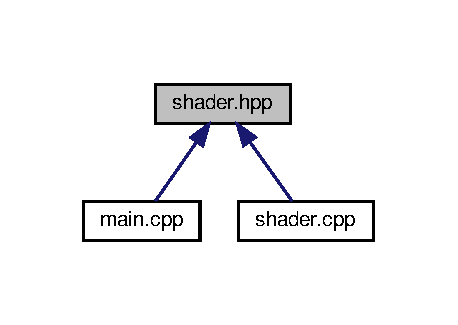
\includegraphics[width=220pt]{shader_8hpp__dep__incl}
\end{center}
\end{figure}
\subsection*{Functions}
\begin{DoxyCompactItemize}
\item 
G\+Luint \hyperlink{shader_8hpp_a833f10cca6a76fe34ae9efa23ac5e73c}{Load\+Shaders} (const char $\ast$vertex\+\_\+file\+\_\+path, const char $\ast$fragment\+\_\+file\+\_\+path)
\end{DoxyCompactItemize}


\subsection{Function Documentation}
\mbox{\Hypertarget{shader_8hpp_a833f10cca6a76fe34ae9efa23ac5e73c}\label{shader_8hpp_a833f10cca6a76fe34ae9efa23ac5e73c}} 
\index{shader.\+hpp@{shader.\+hpp}!Load\+Shaders@{Load\+Shaders}}
\index{Load\+Shaders@{Load\+Shaders}!shader.\+hpp@{shader.\+hpp}}
\subsubsection{\texorpdfstring{Load\+Shaders()}{LoadShaders()}}
{\footnotesize\ttfamily G\+Luint Load\+Shaders (\begin{DoxyParamCaption}\item[{const char $\ast$}]{vertex\+\_\+file\+\_\+path,  }\item[{const char $\ast$}]{fragment\+\_\+file\+\_\+path }\end{DoxyParamCaption})}


\hypertarget{simulTimer_8cpp}{}\section{simul\+Timer.\+cpp File Reference}
\label{simulTimer_8cpp}\index{simul\+Timer.\+cpp@{simul\+Timer.\+cpp}}
{\ttfamily \#include \char`\"{}simul\+Timer.\+h\char`\"{}}\newline
{\ttfamily \#include $<$G\+L\+F\+W/glfw3.\+h$>$}\newline
Include dependency graph for simul\+Timer.\+cpp\+:
\nopagebreak
\begin{figure}[H]
\begin{center}
\leavevmode
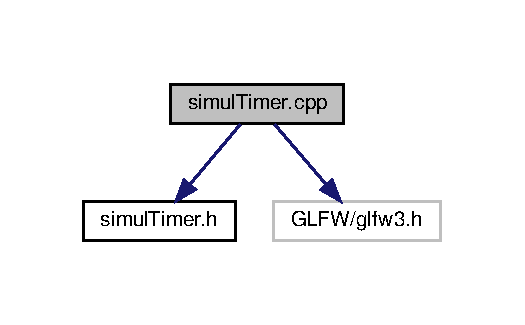
\includegraphics[width=252pt]{simulTimer_8cpp__incl}
\end{center}
\end{figure}

\hypertarget{simulTimer_8h}{}\section{simul\+Timer.\+h File Reference}
\label{simulTimer_8h}\index{simul\+Timer.\+h@{simul\+Timer.\+h}}
This graph shows which files directly or indirectly include this file\+:
\nopagebreak
\begin{figure}[H]
\begin{center}
\leavevmode
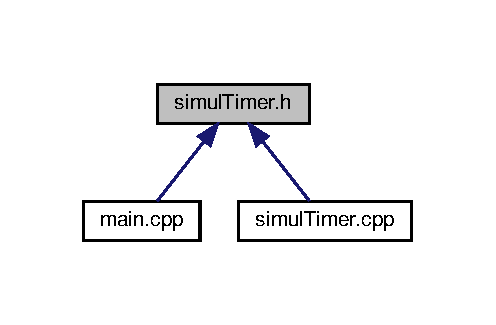
\includegraphics[width=238pt]{simulTimer_8h__dep__incl}
\end{center}
\end{figure}
\subsection*{Classes}
\begin{DoxyCompactItemize}
\item 
class \hyperlink{classsimulTimer}{simul\+Timer}
\end{DoxyCompactItemize}

\hypertarget{texture_8cpp}{}\section{texture.\+cpp File Reference}
\label{texture_8cpp}\index{texture.\+cpp@{texture.\+cpp}}
{\ttfamily \#include $<$stdio.\+h$>$}\newline
{\ttfamily \#include $<$stdlib.\+h$>$}\newline
{\ttfamily \#include $<$string.\+h$>$}\newline
{\ttfamily \#include $<$G\+L/glew.\+h$>$}\newline
{\ttfamily \#include $<$G\+L\+F\+W/glfw3.\+h$>$}\newline
Include dependency graph for texture.\+cpp\+:
\nopagebreak
\begin{figure}[H]
\begin{center}
\leavevmode
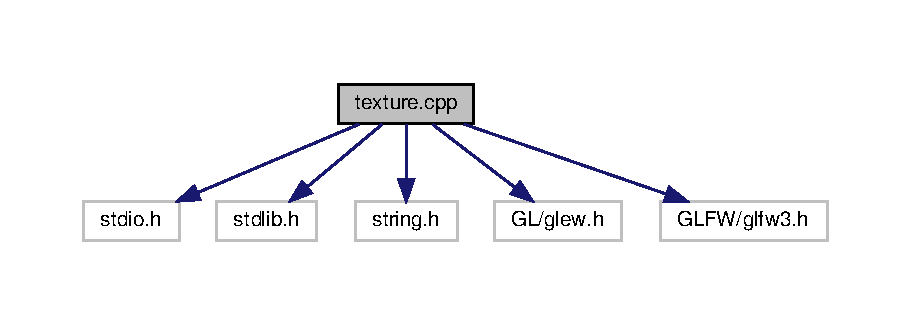
\includegraphics[width=350pt]{texture_8cpp__incl}
\end{center}
\end{figure}
\subsection*{Macros}
\begin{DoxyCompactItemize}
\item 
\#define \hyperlink{texture_8cpp_a468857dac4f79c2eb726895c76a86edb}{F\+O\+U\+R\+C\+C\+\_\+\+D\+X\+T1}~0x31545844
\item 
\#define \hyperlink{texture_8cpp_aff8dbd1cbf63d33501078e742401d01a}{F\+O\+U\+R\+C\+C\+\_\+\+D\+X\+T3}~0x33545844
\item 
\#define \hyperlink{texture_8cpp_a2608b4713fde494b66329c624975a613}{F\+O\+U\+R\+C\+C\+\_\+\+D\+X\+T5}~0x35545844
\end{DoxyCompactItemize}
\subsection*{Functions}
\begin{DoxyCompactItemize}
\item 
G\+Luint \hyperlink{texture_8cpp_a5705f2db49cf4dc13de9d4718e70f8c7}{load\+B\+M\+P\+\_\+custom} (const char $\ast$imagepath)
\item 
G\+Luint \hyperlink{texture_8cpp_a0504d0a1eee3f966798206ee6df63629}{load\+D\+DS} (const char $\ast$imagepath)
\end{DoxyCompactItemize}


\subsection{Macro Definition Documentation}
\mbox{\Hypertarget{texture_8cpp_a468857dac4f79c2eb726895c76a86edb}\label{texture_8cpp_a468857dac4f79c2eb726895c76a86edb}} 
\index{texture.\+cpp@{texture.\+cpp}!F\+O\+U\+R\+C\+C\+\_\+\+D\+X\+T1@{F\+O\+U\+R\+C\+C\+\_\+\+D\+X\+T1}}
\index{F\+O\+U\+R\+C\+C\+\_\+\+D\+X\+T1@{F\+O\+U\+R\+C\+C\+\_\+\+D\+X\+T1}!texture.\+cpp@{texture.\+cpp}}
\subsubsection{\texorpdfstring{F\+O\+U\+R\+C\+C\+\_\+\+D\+X\+T1}{FOURCC\_DXT1}}
{\footnotesize\ttfamily \#define F\+O\+U\+R\+C\+C\+\_\+\+D\+X\+T1~0x31545844}

\mbox{\Hypertarget{texture_8cpp_aff8dbd1cbf63d33501078e742401d01a}\label{texture_8cpp_aff8dbd1cbf63d33501078e742401d01a}} 
\index{texture.\+cpp@{texture.\+cpp}!F\+O\+U\+R\+C\+C\+\_\+\+D\+X\+T3@{F\+O\+U\+R\+C\+C\+\_\+\+D\+X\+T3}}
\index{F\+O\+U\+R\+C\+C\+\_\+\+D\+X\+T3@{F\+O\+U\+R\+C\+C\+\_\+\+D\+X\+T3}!texture.\+cpp@{texture.\+cpp}}
\subsubsection{\texorpdfstring{F\+O\+U\+R\+C\+C\+\_\+\+D\+X\+T3}{FOURCC\_DXT3}}
{\footnotesize\ttfamily \#define F\+O\+U\+R\+C\+C\+\_\+\+D\+X\+T3~0x33545844}

\mbox{\Hypertarget{texture_8cpp_a2608b4713fde494b66329c624975a613}\label{texture_8cpp_a2608b4713fde494b66329c624975a613}} 
\index{texture.\+cpp@{texture.\+cpp}!F\+O\+U\+R\+C\+C\+\_\+\+D\+X\+T5@{F\+O\+U\+R\+C\+C\+\_\+\+D\+X\+T5}}
\index{F\+O\+U\+R\+C\+C\+\_\+\+D\+X\+T5@{F\+O\+U\+R\+C\+C\+\_\+\+D\+X\+T5}!texture.\+cpp@{texture.\+cpp}}
\subsubsection{\texorpdfstring{F\+O\+U\+R\+C\+C\+\_\+\+D\+X\+T5}{FOURCC\_DXT5}}
{\footnotesize\ttfamily \#define F\+O\+U\+R\+C\+C\+\_\+\+D\+X\+T5~0x35545844}



\subsection{Function Documentation}
\mbox{\Hypertarget{texture_8cpp_a5705f2db49cf4dc13de9d4718e70f8c7}\label{texture_8cpp_a5705f2db49cf4dc13de9d4718e70f8c7}} 
\index{texture.\+cpp@{texture.\+cpp}!load\+B\+M\+P\+\_\+custom@{load\+B\+M\+P\+\_\+custom}}
\index{load\+B\+M\+P\+\_\+custom@{load\+B\+M\+P\+\_\+custom}!texture.\+cpp@{texture.\+cpp}}
\subsubsection{\texorpdfstring{load\+B\+M\+P\+\_\+custom()}{loadBMP\_custom()}}
{\footnotesize\ttfamily G\+Luint load\+B\+M\+P\+\_\+custom (\begin{DoxyParamCaption}\item[{const char $\ast$}]{imagepath }\end{DoxyParamCaption})}

\mbox{\Hypertarget{texture_8cpp_a0504d0a1eee3f966798206ee6df63629}\label{texture_8cpp_a0504d0a1eee3f966798206ee6df63629}} 
\index{texture.\+cpp@{texture.\+cpp}!load\+D\+DS@{load\+D\+DS}}
\index{load\+D\+DS@{load\+D\+DS}!texture.\+cpp@{texture.\+cpp}}
\subsubsection{\texorpdfstring{load\+D\+D\+S()}{loadDDS()}}
{\footnotesize\ttfamily G\+Luint load\+D\+DS (\begin{DoxyParamCaption}\item[{const char $\ast$}]{imagepath }\end{DoxyParamCaption})}


\hypertarget{texture_8hpp}{}\section{texture.\+hpp File Reference}
\label{texture_8hpp}\index{texture.\+hpp@{texture.\+hpp}}
This graph shows which files directly or indirectly include this file\+:
\nopagebreak
\begin{figure}[H]
\begin{center}
\leavevmode
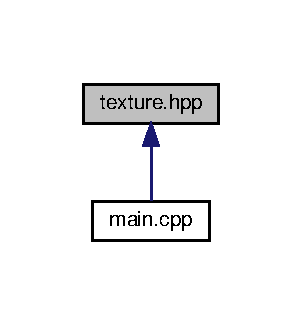
\includegraphics[width=145pt]{texture_8hpp__dep__incl}
\end{center}
\end{figure}
\subsection*{Functions}
\begin{DoxyCompactItemize}
\item 
G\+Luint \hyperlink{texture_8hpp_a5705f2db49cf4dc13de9d4718e70f8c7}{load\+B\+M\+P\+\_\+custom} (const char $\ast$imagepath)
\item 
G\+Luint \hyperlink{texture_8hpp_a0504d0a1eee3f966798206ee6df63629}{load\+D\+DS} (const char $\ast$imagepath)
\end{DoxyCompactItemize}


\subsection{Function Documentation}
\mbox{\Hypertarget{texture_8hpp_a5705f2db49cf4dc13de9d4718e70f8c7}\label{texture_8hpp_a5705f2db49cf4dc13de9d4718e70f8c7}} 
\index{texture.\+hpp@{texture.\+hpp}!load\+B\+M\+P\+\_\+custom@{load\+B\+M\+P\+\_\+custom}}
\index{load\+B\+M\+P\+\_\+custom@{load\+B\+M\+P\+\_\+custom}!texture.\+hpp@{texture.\+hpp}}
\subsubsection{\texorpdfstring{load\+B\+M\+P\+\_\+custom()}{loadBMP\_custom()}}
{\footnotesize\ttfamily G\+Luint load\+B\+M\+P\+\_\+custom (\begin{DoxyParamCaption}\item[{const char $\ast$}]{imagepath }\end{DoxyParamCaption})}

\mbox{\Hypertarget{texture_8hpp_a0504d0a1eee3f966798206ee6df63629}\label{texture_8hpp_a0504d0a1eee3f966798206ee6df63629}} 
\index{texture.\+hpp@{texture.\+hpp}!load\+D\+DS@{load\+D\+DS}}
\index{load\+D\+DS@{load\+D\+DS}!texture.\+hpp@{texture.\+hpp}}
\subsubsection{\texorpdfstring{load\+D\+D\+S()}{loadDDS()}}
{\footnotesize\ttfamily G\+Luint load\+D\+DS (\begin{DoxyParamCaption}\item[{const char $\ast$}]{imagepath }\end{DoxyParamCaption})}


%--- End generated contents ---

% Index
\backmatter
\newpage
\phantomsection
\clearemptydoublepage
\addcontentsline{toc}{chapter}{Index}
\printindex

\end{document}
